\documentclass[preprint,12pt]{elsarticle}
\usepackage{amsmath,amssymb,amsthm}
\usepackage{booktabs,graphicx,multirow,xcolor}
\usepackage[hidelinks]{hyperref}
\providecommand{\detSucc}{--}\providecommand{\detFall}{--}\providecommand{\detTime}{--}\providecommand{\detN}{--}
\providecommand{\enstSucc}{--}\providecommand{\enstFall}{--}\providecommand{\enstTime}{--}\providecommand{\enstN}{--}
\providecommand{\gaussSucc}{--}\providecommand{\gaussFall}{--}\providecommand{\gaussTime}{--}\providecommand{\gaussN}{--}
\newcommand{\detN}{733}
\newcommand{\detSucc}{0.681}
\newcommand{\detFall}{0.319}
\newcommand{\detTime}{0.000}
\newcommand{\enstN}{768}
\newcommand{\enstSucc}{0.656}
\newcommand{\enstFall}{0.344}
\newcommand{\enstTime}{0.000}
\newcommand{\gaussN}{285}
\newcommand{\gaussSucc}{0.758}
\newcommand{\gaussFall}{0.088}
\newcommand{\gaussTime}{0.154}
\newcommand{\esolN}{288}
\newcommand{\esolSucc}{0.757}
\newcommand{\esolFall}{0.101}
\newcommand{\esolTime}{0.142}
\newcommand{\escrnN}{329}
\newcommand{\escrnSucc}{0.888}
\newcommand{\escrnFall}{0.033}
\newcommand{\escrnTime}{0.079}
\newcommand{\esfbN}{377}
\newcommand{\esfbSucc}{0.902}
\newcommand{\esfbFall}{0.069}
\newcommand{\esfbTime}{0.029}
\newcommand{\esfbcrnN}{398}
\newcommand{\esfbcrnSucc}{0.925}
\newcommand{\esfbcrnFall}{0.043}
\newcommand{\esfbcrnTime}{0.033}

\journal{TBD}

\begin{document}
\begin{frontmatter}

\title{Planning with stochastic latent world models: distributional predictors, coupled noise and feedback}

\author[buv]{Quang-Vinh Dang\corref{cor1}}
\ead{vinh.dq4@buv.edu.vn}
\cortext[cor1]{Corresponding author. ORCID: 0000-0002-3877-8024}
\address[buv]{British University Vietnam, Hung Yen, Vietnam}

\begin{abstract}
Decoder-free latent world models such as LeWorldModel plan by rolling a deterministic predictor forward and minimising the latent distance to a goal embedding.
When the dynamics are stochastic, a deterministic predictor learns the conditional mean, which can correspond to no reachable state, and the planner cannot see the tail events that decide success.
We study sampling-based planning with stochastic latent predictors on a controlled hazard-navigation benchmark in which the true simulator provides a reference.
Replacing the deterministic predictor by a distributional one trained with the energy score, and averaging the planning cost over noise particles, raises the success rate from \detSucc{} to \esolSucc{} and lowers the fall rate from \detFall{} to \esolFall{} at the same horizon and candidate budget.
Two classical devices then account for most of the remaining gap to the simulator-based planner: sharing the noise across candidates and across replans (common random numbers) mainly removes falls, and parameterising each plan as nominal actions plus a feedback gain on the deviation of the sampled latent from its noise-free rollout mainly removes timeouts.
Together they reach success \esfbcrnSucc{}, fall \esfbcrnFall{} and timeout \esfbcrnTime{} for 12.5\,\% extra compute.
We give elementary results that explain each effect (a regret identity for mean-embedding planning, tail blindness amplified by selection, a strict open-loop gap with an absorbing boundary) and report negative results for risk-averse scoring, empirical-Bayes shrinkage, particle racing, importance sampling, failure-rate control and several test-time adaptation schemes.
The benchmark is low-dimensional and uses a frozen encoder; we discuss why, and what this limits.
\end{abstract}

\begin{keyword}
world models \sep model predictive control \sep stochastic dynamics \sep energy score \sep common random numbers \sep feedback planning
\end{keyword}
\end{frontmatter}

% =====================================================================================================
\section{Introduction}\label{sec:intro}

Joint-embedding predictive architectures (JEPAs) have become a practical way to learn world models for control without reconstructing pixels.
Recent systems plan with a frozen encoder and a deterministic latent predictor: a population-based optimiser such as the cross-entropy method (CEM) proposes action sequences, the predictor is rolled out, and the sequence whose final embedding is closest to the goal embedding is executed~\cite{zhou2024dinowm,maes2026lewm}.
The predictor is trained with a mean-squared loss, so it estimates the conditional mean embedding.
The authors of the JEPA-WM study note that environments with aleatoric uncertainty would require stochastic predictors~\cite{terver2025jepawm}.

This matters when the dynamics have rare but costly outcomes.
Consider an agent that must cross a region next to a pit while a random wind pushes it sideways.
Averaged over the wind, the predicted next state is the same for a path hugging the pit edge and for a path that keeps a safe distance, so a deterministic planner prefers the shorter, riskier one.
The planner is not wrong about the average; it is blind to the spread.
Figure~\ref{fig:benchmark} shows this on the benchmark used in this paper.

Stochastic and distributional JEPA predictors have appeared recently.
Branch-JEPA trains a set of weighted latent successors with the energy score~\cite{branchjepa2026}, a variational JEPA writes the stochastic model-predictive objective~\cite{vjepa2026}, and a flow-matching predictor has been combined with CEM on LeWorldModel using one generated sample per candidate~\cite{flowjepa2026}.
What is missing, to our knowledge, is a controlled comparison of what a planner needs, beyond a stochastic predictor, to profit from it: how many particles, how to rank candidates with them, and whether the open-loop plan that CEM optimises is the right object when the agent replans with feedback every step.
This paper provides such a comparison on a benchmark with a known reference.

\paragraph{Contributions.}
\begin{enumerate}
\item A stochastic hazard-navigation benchmark with a true-simulator reference planner, an exemplar-based failure detector that works in latent space, and a protocol with confidence intervals (Section~\ref{sec:setting}).
\item A controlled comparison of deterministic, Gaussian, energy-score and ensemble predictors under identical planners (Section~\ref{sec:exp}). A distributional predictor with particle-averaged cost raises success by \esolSuccDiff{} points and cuts falls by a factor of about three relative to the deterministic planner; an ensemble of deterministic predictors does not help.
\item Two components, both classical, whose effect in this setting we measure and explain: common random numbers shared across candidates and chained across replans (Section~\ref{sec:crn}), and a feedback-parameterised CEM (Section~\ref{sec:fb}). Their combination closes most of the gap to the simulator-based planner at 12.5\,\% extra compute.
\item Elementary theory that explains each effect, verified numerically (Section~\ref{sec:theorysummary}, Appendix~\ref{sec:theory}).
\item A set of negative results (Section~\ref{sec:negative}) that save others the same experiments: risk-averse scoring, empirical-Bayes shrinkage, racing, noise-space importance sampling, failure-rate control, spread recalibration and online fine-tuning did not improve on plain expected-cost planning in our setting.
\end{enumerate}

\paragraph{What we do not claim.}
Common random numbers, feedback policies inside model-predictive control, and energy-score training all have long histories (Section~\ref{sec:related}); we do not claim them as new.
We claim a measurement of how much each matters for planning with stochastic decoder-free latent predictors, the explanation, and the negative results.
Our experiments are small-scale (a two-dimensional point agent, a frozen identity encoder, CPU); Section~\ref{sec:limits} states what this does and does not support.

% =====================================================================================================
\section{Related Work}
\label{sec:related}

\paragraph{Latent world models for planning.}
Learning a compact latent model of the environment and using it for control goes back to World Models~\cite{ha2018world}, PlaNet~\cite{hafner2019planet} and the Dreamer line~\cite{hafner2020dreamer,hafner2021dreamerv2,hafner2025dreamerv3,hafner2025dreamer4}, which train behaviours by actor-critic learning on imagined latent rollouts. Transformer and diffusion world models follow the same recipe in discrete or pixel space~\cite{micheli2023iris,alonso2024diamond}, and JEDI trains a diffusion world model end to end with a JEPA-style latent objective for online reinforcement learning, explicitly without look-ahead planning~\cite{lim2026jedi}. TD-MPC and TD-MPC2 instead plan online with MPPI~\cite{williams2016mppi} in a decoder-free latent space~\cite{hansen2022tdmpc,hansen2024tdmpc2}. Model-based methods with probabilistic ensembles~\cite{chua2018pets,janner2019mbpo,yu2020mopo} are the classical antecedent for treating model uncertainty during planning. Recent surveys cover the wider field~\cite{zidan2026survey,hou2026robotsurvey}.

\paragraph{JEPA world models and their planning objective.}
Joint-embedding predictive architectures predict in representation space rather than pixel space~\cite{assran2023ijepa,bardes2024vjepa}. Action-conditioned variants give zero-shot goal-reaching by planning with a frozen predictor: DINO-WM on pretrained patch features~\cite{zhou2024dinowm}, PLDM on reward-free offline data~\cite{sobal2025pldm}, V-JEPA~2 at video scale~\cite{assran2025vjepa2}, and LeWorldModel (LeWM), which trains an encoder and predictor from pixels with a prediction loss and the SIGReg regulariser of LeJEPA~\cite{maes2026lewm,balestriero2025lejepa}. The design space of this family is mapped in~\cite{terver2025jepawms}, and \texttt{stable-worldmodel} provides shared environments and planners~\cite{maes2026swm}. All of these use a deterministic predictor and rank candidate action sequences by the distance between the predicted terminal latent and the goal latent, usually with CEM~\cite{rubinstein1999cem}.

A fast-growing set of 2026 papers argues that this planning objective is the weak point. The latent distance can correlate poorly with true cost, saturate, or invert at long range~\cite{singh2026objective}, and frozen JEPA objectives can rank candidate actions incorrectly even when closed-loop replanning hides it~\cite{zhang2026arcbench,wang2026decisionmetric,chen2026atm}. Proposed repairs replace or augment the cost with learned temporal or reachability metrics~\cite{li2026trm,bai2026tdjepa,fu2026cgs}, retrieve anchors from offline trajectories~\cite{liu2026anchored}, improve proposals with subgoals~\cite{cheng2026sage}, or learn decision-aligned relations among candidates~\cite{liu2026djepa}. Alrasheed et al.\ study the rollout horizon at which frozen-backbone predictors stop ranking actions reliably~\cite{alrasheed2026limits}. Li et al.\ describe proposal overgeneration: when predicted terminal costs carry residual error, enlarging the candidate pool lowers the feasibility of the minimum-cost candidate~\cite{li2026overgeneration}. This is a selection effect of the kind studied as the optimizer's curse~\cite{smith2006optimizers}, reward-model overoptimization~\cite{gao2023overopt,khalaf2025inferencehacking} and model exploitation~\cite{bhamidipaty2026exploitable}. Our work keeps the distance cost fixed and varies the predictor and how the planner uses it.

\paragraph{Stochastic and distributional world models.}
Stochastic latent states have long been standard in recurrent world models~\cite{hafner2019planet,hafner2025dreamerv3}, whereas the JEPA planners above are deterministic. Several recent papers make the JEPA predictor probabilistic. VJEPA gives a variational formulation, proves that its latent can be a sufficient information state for control, writes the stochastic MPC objective (expected cost under the predictive distribution) and a sampling-based latent MPC routine, and validates on a linear-Gaussian ``noisy TV'' toy~\cite{huang2026vjepa}; it also proves that mean planning is optimal when the predictive covariance does not depend on the action and the cost is quadratic. Var-JEPA gives a related ELBO view~\cite{gogl2026varjepa}. Branch-JEPA represents the transition as a finite set of weighted latent successors trained with the energy score, and is evaluated by offline trajectory forecasting on Argoverse~2 rather than closed-loop control~\cite{song2026branchjepa}. Flow-JEPA replaces LeWM's regression predictor with a flow-matching trajectory generator and plans with CEM, motivated by robustness to visual noise; as described, each candidate is scored with one generated future~\cite{huo2026flowjepa}. FlowWM performs flow matching in pretrained feature space and is evaluated on forecasting and perception benchmarks~\cite{porcher2026flowwm}. Dong proves that observed transitions cannot separate state aliasing from process noise~\cite{dong2026closure}. Training a predictor on a proper scoring rule~\cite{gneiting2007scoring} is standard in probabilistic forecasting: engression fits generative models with the energy score~\cite{shen2025engression}, and AIFS-CRPS trains an operational weather ensemble on the CRPS~\cite{lang2024aifscrps}. Deep ensembles are the other common route to predictive distributions~\cite{lakshminarayanan2017ensembles,chua2018pets}.

\paragraph{Risk-aware planning with learned models.}
PETS propagates particles through a probabilistic ensemble and optimises expected return with MPC~\cite{chua2018pets}; MOPO penalises model uncertainty in offline reinforcement learning~\cite{yu2020mopo}. Risk-sensitive sampling-based MPC uses the conditional value-at-risk~\cite{rockafellar2000cvar} inside MPPI~\cite{yin2022ramppi,enwerem2026riskbelief}, and particle MPC treats any particle representation of uncertainty as a set of scenarios~\cite{dyro2021pmpc}. In latent world models, safety is pursued by conformal error bounds inside robust MPC~\cite{nath2026sls}, by safe reinforcement learning inside world models~\cite{huang2024safedreamer}, and by adaptive latent safety filters~\cite{cao2026worldmodelslie}. D-JEPA includes expected-value and CVaR planning over 16 sampled futures per candidate among its baselines, with nearly identical scores~\cite{liu2026djepa}. Estimating failure probabilities of candidate plans by importance sampling is established in motion planning~\cite{janson2017mcmp,schmerling2017adaptiveis}. For choosing among noisy candidates, the simulation literature offers ranking and selection procedures~\cite{kim2001fully}, racing~\cite{maron1993hoeffding}, and common random numbers~\cite{glasserman1992crn}, and the statistics literature offers empirical-Bayes shrinkage~\cite{efron1973stein}. These tools are standard and we apply them as add-ons to latent planning, so the question we ask is whether they help there.

\paragraph{Test-time adaptation and calibration.}
Adapting a model at test time from a self-supervised signal is well established~\cite{sun2020ttt,wang2021tent}. For latent world models, AdaJEPA updates the predictor inside the MPC loop from observed transitions~\cite{wang2026adajepa}, JEPA-TTT accumulates updates across episodes~\cite{zhang2026jepattt}, and Sandwich-Residuals learns small residual corrections around a frozen predictor~\cite{soni2026sandwich}. All three adapt a deterministic predictor. Adaptive conformal inference~\cite{gibbs2021aci} and conformal decision theory~\cite{lekeufack2024cdt} recalibrate prediction sets or decision parameters online under shift and are the natural tools for recalibrating the spread of a distributional predictor.

\paragraph{Positioning.}
Much of what we use has precedent, and we do not claim it as new. Planning with particles through a probabilistic model is PETS~\cite{chua2018pets}. The stochastic latent MPC objective and a sampling-based planner for JEPA predictors appear in VJEPA~\cite{huang2026vjepa}. Energy-score training of a JEPA predictor appears in Branch-JEPA~\cite{song2026branchjepa}. A generative JEPA predictor planned with CEM on top of LeWM appears in Flow-JEPA~\cite{huo2026flowjepa}. CVaR and expected-value scoring over sampled latent futures appear as baselines in~\cite{liu2026djepa}. The present paper is a controlled study of stochastic latent planning in this setting. We compare deterministic and distributional predictors under the same particle-based planner, on a benchmark with planted stochastic hazards, together with a theoretical account of when planning with a distribution can differ from planning with its mean, and a set of negative results on popular add-ons (risk-averse scoring, shrinkage, racing, common random numbers, importance sampling, and test-time adaptation).

To our knowledge, none of the closed-loop JEPA-planning papers above trains a predictor with a proper scoring rule and evaluates particle-averaged planning against a matched deterministic predictor, and none studies the add-ons listed above systematically. This statement rests on searches of arXiv titles and abstracts and of the web up to 5 October 2026, so it can fail for work we could not find, and it concerns only this combination, not its individual ingredients.


% =====================================================================================================
\section{Problem setting and benchmark}\label{sec:setting}

\paragraph{Planning problem.}
An agent with state $s_t$ acts with $a_t$; the world is stochastic.
A latent world model consists of an encoder $\phi$ and a predictor $z_{t+1}=f(z_t,a_t,u_t)$ with noise $u_t\sim\mathcal N(0,I)$ (a deterministic predictor ignores $u_t$).
Given the encoded current observation $z_0=\phi(o_0)$ and a goal embedding $z_g=\phi(o_g)$, a planner chooses an action sequence $a_{0:H-1}$ by minimising the expected planning cost
\begin{equation}\label{eq:cost}
J(a)=\mathbb E_u\Big[\tfrac1{s_0}\Big(\|z_H-z_g\|^2+\tfrac1H\textstyle\sum_{t=1}^{H}\|z_t-z_g\|^2\Big)+\kappa\,\mathbf 1\{\text{failure}\}\Big],
\end{equation}
estimated with $M$ noise particles per candidate; $s_0$ is the median squared start--goal latent distance (a normalisation) and $\kappa=3$.
The planner executes the first action and replans at every step.

\paragraph{Failure detection in latent space.}
The failure event is specified by exemplar frames, in the same way the goal is specified by an image.
We encode a labelled sample of failure frames, take their mean embedding as an anchor, and call a latent state a failure if its squared distance to the anchor is below a threshold chosen to maximise accuracy on labelled data (0.999 for the main model).
The same detector and the same $\kappa$ are used for every planner.

\paragraph{Benchmark.}
A point agent moves in the unit square, $p_{t+1}=\mathrm{clip}(p_t+0.05\,a_t+w_t e_y)$ with $a_t\in[-1,1]^2$ and wind $w_t=\pm w$ with equal probability.
An absorbing pit occupies $[0.25,0.75]\times[0,0.30]$; start and goal lie on opposite sides at heights $y\in[0.34,0.46]$ and the straight path crosses the edge of the pit.
The main variant uses $w=0.09$; because $w$ exceeds the agent's own authority (0.05 per step) the agent cannot cancel the wind and must keep a margin.
An episode ends with success (distance to goal below 0.06), fall (entering the pit), or timeout (120 steps).
Episodes restart on termination; 16 environments run in parallel.
Planning settings are $N=32$ candidates, $M=8$ particles, horizon $H=10$, three CEM iterations, unless stated.
A reference planner that uses the true simulator as its model (large budget: $N=64$, $M=12$, $H=12$) is reported as an upper bound.

\paragraph{World models.}
The encoder is a frozen identity map on $(2x-1,2y-1,f)$, where $f$ marks a fallen state, so the latent metric is faithful by construction.
We freeze it because encoders learned end-to-end with the SIGReg regulariser~\cite{maes2026lewm,balestriero2025lejepa} produced latent distances that correlate poorly with true distance at our scale (Spearman 0.44--0.76 against 1.00 for the frozen map, Section~\ref{sec:negative}); this confound would hide the effect we want to study.
The predictors are MLPs ($3\times512$, LayerNorm) trained for 8\,000 steps on $3\times10^5$ transitions with 25\,\% of the data collected in a band next to the pit.
We compare: (i) \emph{deterministic} (mean-squared loss, mean rollout, as in LeWorldModel); (ii) \emph{ensemble} of three deterministic predictors, one member per particle (epistemic spread only); (iii) \emph{Gaussian} head with diagonal covariance (negative log-likelihood); (iv) \emph{energy-score} predictor with an 8-dimensional noise input, trained with the unbiased energy score on $8$ samples per transition.
Three independent model seeds are trained per kind.

\begin{figure}[t]
\centering
\includegraphics[width=0.92\linewidth]{figs/benchmark}
\caption{The benchmark. Ten episodes planned with the true simulator, once with a deterministic (mean) rollout and once with particle-averaged cost. Orange paths end in the pit (cross); blue paths reach the goal side. The mean rollout sees no difference between hugging the pit edge and keeping a margin.}
\label{fig:benchmark}
\end{figure}

\paragraph{Protocol and statistics.}
All planner comparisons in Section~\ref{sec:exp} use the same environment stream (evaluation seed 211), three model seeds and 450 steps per run, which gives 290--400 episodes per planner.
Intervals are 95\,\% bootstrap (or Wilson) intervals over episodes; episodes within a run are not exactly independent, so the intervals are somewhat optimistic.
Differences below about 0.06 in a rate cannot be resolved at this sample size and we do not interpret them.

% =====================================================================================================
\section{Planning with stochastic predictors}\label{sec:methods}

\subsection{Particle-based CEM}\label{sec:pcem}
The baseline planner is standard CEM over action sequences with $M$ particles per candidate: sample $N$ sequences from a diagonal Gaussian, roll each of them out $M$ times with independent noise, score by the particle mean of~\eqref{eq:cost}, refit the Gaussian to the best 10\,\%, and repeat.

\subsection{Coupled noise}\label{sec:crn}
With independent noise, each candidate is scored on its own $M$ draws.
A candidate that passes close to the hazard has a rare, expensive tail; with few particles the tail is often not drawn, and selecting the minimum over candidates then favours exactly the candidates whose tail was missed (Section~\ref{sec:theorysummary}).
Common random numbers (CRN) draw one noise tensor and use it for every candidate, so that the noise error cancels in the comparison between candidates~\cite{glasserman1992crn}.
We use two variants: \emph{CRN} (one tensor per planning call, redrawn at every CEM iteration) and \emph{chained CRN}, where the tensor of the previous replan is shifted by one step and mixed with fresh noise, $u\leftarrow\sqrt{1-r^2}\,u_{\mathrm{old}}+r\,\varepsilon$ with $r=0.3$, so that consecutive replans see consistent scenarios.
Antithetic pairs and scrambled Sobol sequences were also tested and added little once the noise was shared (Section~\ref{sec:exp}).

\subsection{Feedback-parameterised CEM}\label{sec:fb}
CEM optimises an open-loop sequence against random noise, but the agent will replan with feedback after one step.
We parameterise each candidate as nominal actions plus a diagonal feedback law on the deviation of the sampled latent state from the noise-free rollout of the same predictor,
\begin{equation}\label{eq:fb}
a_t=\mathrm{clip}\big(a^{\mathrm{nom}}_t+K_t\,(z_t-\bar z_t)_{xy}\big),\qquad \bar z_{t+1}=f(\bar z_t,a^{\mathrm{nom}}_t,0),
\end{equation}
with one gain per axis and time step, $K_t\in[-k_{\max},0]$, and CEM samples and refits $(a^{\mathrm{nom}},K)$ jointly.
Only $a^{\mathrm{nom}}_0$ is executed, since the deviation is zero at $t=0$.
The form is that of tube MPC and affine disturbance feedback; what is specific to the present setting is that $\bar z$ exists because the predictor is stochastic and decoder-free.
The overhead is one extra predictor evaluation per candidate and step, i.e.\ $1/M$ of the particle cost (12.5\,\% for $M=8$).

% =====================================================================================================
\section{Why the effects occur}\label{sec:theorysummary}

Appendix~\ref{sec:theory} states and proves each result and lists the numerical check that accompanies it.
We summarise the three that explain the experiments.
Our results are elementary; they are meant to explain, not to be deep, and ``new'' in the appendix means new in this form for the planning setting.

\paragraph{Mean-embedding planning ignores the spread.}
For the squared-distance cost, $\mathbb E\|Z-g\|^2=\|\mu-g\|^2+\operatorname{tr}\Sigma$, and a mean-squared-error predictor converges to $\mu$.
The regret of the deterministic planner for the expected cost equals the difference of the noise premiums $\operatorname{tr}\Sigma$ at its choice and at the optimum, and is at most their spread (Theorem~\ref{thm:regret}); it is tight.
It vanishes if the covariance does not depend on the action, which is the case treated by earlier theory~\cite{vjepa2026}; the benchmark here has action-dependent covariance because the noise matters only near the hazard.

\paragraph{Selection amplifies tail blindness.}
Let $N_r$ risky candidates have failure probability $p$ and be cheaper than a safe candidate when no failure is observed.
With $M$ particles per candidate, the planner selects a risky candidate with probability
\begin{equation}
1-\big(1-F_{\mathrm{Bin}}(k^*;M,p)\big)^{N_r},\qquad k^*=\lfloor M(c_s-c_r)/\kappa\rfloor,
\end{equation}
which increases to one with $N_r$ (Theorem~\ref{thm:select}, Figure~\ref{fig:tail}).
Re-evaluating the top candidates on fresh samples removes the selection bias for the final choice (Theorem~\ref{thm:verify}), and, because every shared draw benefits all candidates alike, coupling the noise removes it from the comparison altogether (variance of a cost difference, Proposition~\ref{prop:noisemap}).
A monotone shrinkage of the scores (empirical Bayes) cannot change the argmin when all candidates use the same $M$ (Proposition~\ref{prop:shrink}), which is consistent with its absence of effect in Section~\ref{sec:negative}.

\paragraph{Open-loop plans are strictly worse than closed-loop plans.}
With an absorbing boundary and noise, the best open-loop plan is strictly worse than the best closed-loop plan for every horizon $H\ge2$ (Theorem~\ref{thm:barrier}), and in the linear-quadratic case the open-loop value is $H$ times the closed-loop value (Theorem~\ref{thm:lqg}).
We found that feedback does \emph{not} bound the cumulative probability of reaching the boundary (Remark~\ref{rem:firstpassage}); the benefit in Section~\ref{sec:exp} is faster progress, not safety.

\begin{figure}[t]
\centering
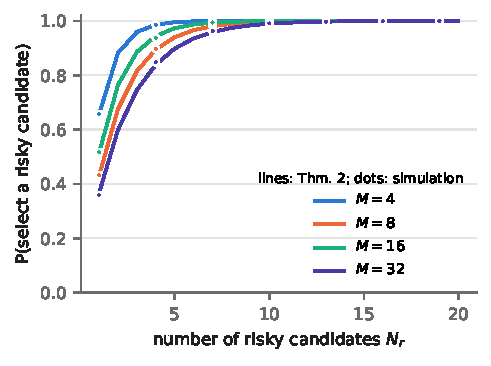
\includegraphics[width=0.55\linewidth]{figs/tail}
\caption{Probability that the planner selects a risky candidate as a function of the number of risky candidates, for different particle counts ($p=0.1$, penalty $\kappa=3$). Lines: Theorem~\ref{thm:select}; dots: simulation.}
\label{fig:tail}
\end{figure}

% =====================================================================================================
\section{Experiments}\label{sec:exp}

\subsection{Predictors and planner components}\label{sec:main}
Table~\ref{tab:main} and Figure~\ref{fig:outcomes} give the main comparison under one protocol.
\begin{table}[t]
\centering\footnotesize
\begin{tabular}{lrcccr}
\toprule
Planner & Episodes & Success & Fall & Timeout & Steps \\
\midrule
Deterministic predictor, mean rollout & 733 & 0.681 \,[0.646,0.713] & 0.319 \,[0.287,0.354] & 0.000 \,[0.000,0.005] & 29 \\
Ensemble of 3 deterministic predictors & 768 & 0.656 \,[0.622,0.689] & 0.344 \,[0.311,0.378] & 0.000 \,[0.000,0.005] & 29 \\
Gaussian predictor, particles & 285 & 0.758 \,[0.705,0.804] & 0.088 \,[0.060,0.126] & 0.154 \,[0.117,0.201] & 58 \\
\midrule
Energy-score predictor, particles (open loop) & 288 & 0.757 \,[0.704,0.803] & 0.101 \,[0.071,0.141] & 0.142 \,[0.107,0.187] & 59 \\
\quad + coupled noise (CRN, chained) & 329 & 0.888 \,[0.849,0.917] & 0.033 \,[0.019,0.059] & 0.079 \,[0.054,0.113] & 51 \\
\quad + feedback gains & 377 & 0.902 \,[0.868,0.928] & 0.069 \,[0.047,0.099] & 0.029 \,[0.016,0.051] & 48 \\
\quad + feedback gains + coupled noise & 398 & 0.925 \,[0.894,0.947] & 0.043 \,[0.027,0.067] & 0.033 \,[0.019,0.055] & 44 \\
\bottomrule
\end{tabular}

\caption{Planners on the benchmark (3 model seeds, same environment stream). Intervals: 95\,\% (Wilson for the first three rows, bootstrap-equivalent for the rest). ``Steps'' is the median number of steps to reach the goal. Reference: the planner that uses the true simulator reaches the success, fall and timeout rates given in Table~\ref{tab:oracle}.}
\label{tab:main}
\end{table}

\begin{figure}[t]
\centering
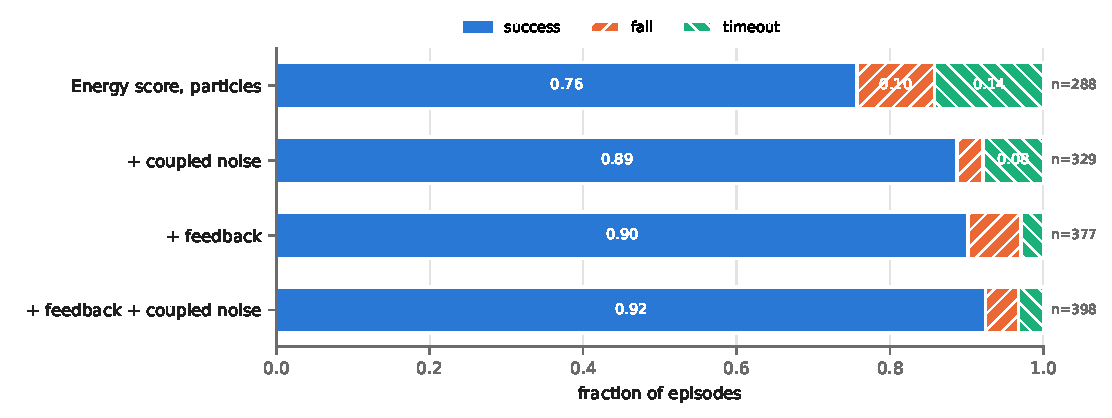
\includegraphics[width=0.95\linewidth]{figs/outcomes}
\caption{Episode outcomes per planner (same data as Table~\ref{tab:main}).}
\label{fig:outcomes}
\end{figure}

\begin{table}[t]
\centering\footnotesize
\begin{tabular}{llcc}
\toprule
Planner & Compute & Wind 0.09 & Wind 0.13 \\
\midrule
Mean-dynamics planning & $N{=}32$, $M{=}8$, $H{=}10$ & 0.322/0.678/0.000 (1826) & 0.237/0.763/0.000 (1811) \\
Particle-averaged planning & $N{=}32$, $M{=}8$, $H{=}10$ & 0.836/0.090/0.074 (458) & 0.752/0.139/0.109 (395) \\
Particle-averaged planning & $N{=}64$, $M{=}12$, $H{=}12$ & 0.874/0.028/0.098 (428) & 0.761/0.097/0.142 (381) \\
\bottomrule
\end{tabular}

\caption{Reference planners that use the true simulator (upper bound), at two compute settings and two wind amplitudes.}
\label{tab:oracle}
\end{table}

\paragraph{Findings.}
\emph{(i) A distributional predictor is the main gain.} Moving from the deterministic predictor (success \detSucc, fall \detFall) to the energy-score predictor with particle-averaged cost (\esolSucc, \esolFall) changes the outcome more than any later component. The Gaussian head is intermediate (\gaussSucc, \gaussFall) and the three-member deterministic ensemble gives no benefit (\enstSucc, \enstFall); the energy-score and Gaussian rows differ by less than we can resolve.
\emph{(ii) Coupled noise removes falls.} Chained CRN lowers the fall rate from \esolFall{} to \escrnFall{} without extra forward passes.
\emph{(iii) Feedback removes timeouts.} Feedback gains lower the timeout rate from \esolTime{} to \esfbTime{} and raise success to \esfbSucc, at 12.5\,\% extra compute.
\emph{(iv) The two are complementary.} Combined, success is \esfbcrnSucc, fall \esfbcrnFall, timeout \esfbcrnTime. The combination is not significantly better than the better component on any single metric, but it is not worse than either.

\subsection{Sample efficiency}\label{sec:sweep}
Figure~\ref{fig:sweep} and Table~\ref{tab:sweep} vary the number of particles per candidate.
With independent noise the success rate does not improve monotonically with $M$ in our runs; with coupled noise and feedback, $M=4$ already exceeds the baseline at $M=8$ and $M=16$ in success, using 3.2 times fewer predictor evaluations than the baseline at $M=16$.
These sweeps use one or two model seeds and about 100--250 episodes per cell, so they are indicative only.

\begin{figure}[t]
\centering
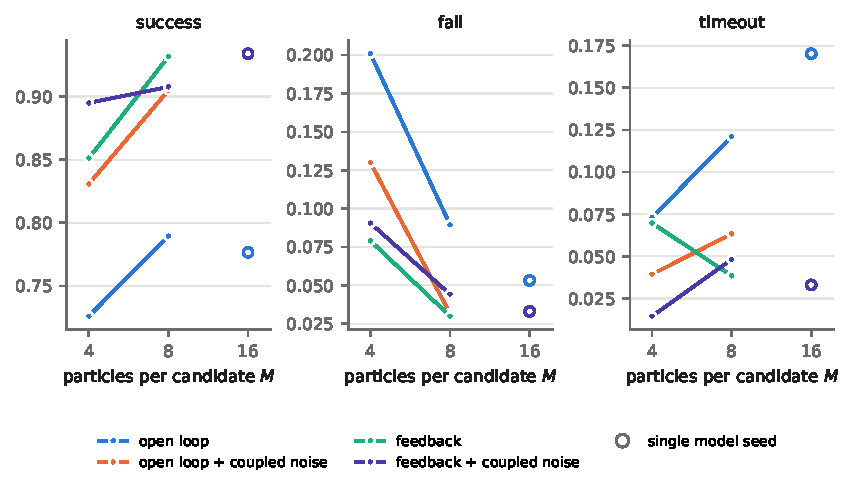
\includegraphics[width=0.98\linewidth]{figs/sweep}
\caption{Effect of the number of particles per candidate. $M=4$ and $M=8$ pool two model seeds; $M=16$ (hollow markers) uses one model seed.}
\label{fig:sweep}
\end{figure}

\begin{table}[t]
\centering\footnotesize
\begin{tabular}{lccc}
\toprule
Planner & $M=4$ & $M=8$ & $M=16$ \\
\midrule
Open loop, independent noise & 0.726/0.201/0.073 (219) & 0.789/0.089/0.121 (190) & 0.777/0.053/0.170 (94, 1 model seed) \\
Open loop, coupled noise & 0.831/0.130/0.039 (254) & 0.905/0.032/0.063 (221) & -- \\
Feedback, independent noise & 0.851/0.079/0.070 (215) & 0.932/0.030/0.038 (234) & -- \\
Feedback, coupled noise & 0.895/0.091/0.014 (276) & 0.908/0.044/0.048 (249) & 0.934/0.033/0.033 (121, 1 model seed) \\
\bottomrule
\end{tabular}

\caption{Success/fall/timeout (episodes) by particle count, same data as Figure~\ref{fig:sweep}.}
\label{tab:sweep}
\end{table}

\subsection{Distribution shift}\label{sec:shift}
We raise the wind amplitude from 0.09 to 0.13 after 200 steps without retraining (Table~\ref{tab:shift}); the true-simulator planner then achieves a success rate of 0.774 and a fall rate of 0.068 (Table~\ref{tab:oracle}).
All learned planners degrade; the distributional predictor degrades much less than the deterministic one, but none of the adaptation schemes we tried closes the gap (Section~\ref{sec:negative}).

\begin{table}[t]
\centering\footnotesize
\begin{tabular}{lrcc|rccc}
\toprule
 & \multicolumn{3}{c}{Before shift} & \multicolumn{4}{c}{After shift} \\
Planner & Eps & Succ. & Fall & Eps & Succ. & Fall & Timeout \\
\midrule
Deterministic predictor, mean rollout & 328 & 0.668 & 0.332 & 631 & 0.399 & 0.601 & 0.000 \\
Energy-score predictor, particles & 116 & 0.828 & 0.086 & 230 & 0.709 & 0.200 & 0.091 \\
\quad CVaR$_{0.5}$ scoring & 90 & 0.678 & 0.067 & 218 & 0.656 & 0.216 & 0.128 \\
\quad failure-rate controller (target 0.05) & 99 & 0.768 & 0.081 & 218 & 0.615 & 0.220 & 0.165 \\
\quad scalar spread recalibration (online) & 107 & 0.822 & 0.047 & 233 & 0.665 & 0.240 & 0.094 \\
\quad per-dimension spread recalibration & 110 & 0.836 & 0.045 & 218 & 0.606 & 0.197 & 0.197 \\
\quad online fine-tuning of the predictor & 145 & 0.717 & 0.234 & 209 & 0.550 & 0.263 & 0.187 \\
\bottomrule
\end{tabular}

\caption{Wind shift from 0.09 to 0.13 at step 200 (models not retrained). Rows below the energy-score planner are variants of it. Each row pools three model seeds; episode counts are small, so differences below about 0.06 are not resolved.}
\label{tab:shift}
\end{table}

% =====================================================================================================
\section{Negative results}\label{sec:negative}

The following were tried on the same benchmark and did not improve on plain expected-cost planning with the energy-score predictor; all numbers come from the files in the repository (\texttt{results/FINDINGS\_stochastic.md}).
\begin{itemize}
\item \emph{Risk-averse scoring.} $\mathrm{CVaR}$ mixed into the score (weights 0.5 and 1.0) lowered neither falls nor raised success, and increased timeouts (0.24 and 0.30 against 0.09). A comparison of expected and CVaR planning over sampled futures with no gain has also been reported for a probabilistic JEPA~\cite{djepa2026}.
\item \emph{Empirical-Bayes shrinkage and racing.} Shrinking candidate scores towards the pool mean and allocating particles by successive halving did not raise success; shrinkage with equal $M$ cannot change the ranking (Proposition~\ref{prop:shrink}).
\item \emph{Noise-space importance sampling.} A mean-shifted Gaussian proposal (gradient or cross-entropy direction) for estimating failure probabilities had higher error than plain Monte Carlo for the gradient shift ($0.21$ to $4.3$ against $0.10$ RMSE) in the 80-dimensional noise space of a ten-step rollout. Importance sampling in noise space for collision probabilities is classical in motion planning~\cite{janson2015mcmp,schmerling2017adaptive}.
\item \emph{Failure-rate control.} An online controller adapting the CVaR weight to hold the observed fall rate at 0.05 saturated at weight 0.92 after the wind shift and left the fall rate at 0.22: when the model is wrong, a risk measure over the wrong distribution cannot restore safety.
\item \emph{Spread recalibration.} Online recalibration of the predictive spread by energy-score gradient descent identified the correct scale (1.37 against the true 1.44 for a scalar; 1.35 for the $y$ component) but did not reduce falls, and setting the oracle scale made them worse.
\item \emph{Online fine-tuning.} Fine-tuning the predictor with its own loss (mean-squared, Gaussian likelihood, energy score) degraded performance before the shift and did not help after it; a drift-gated, replay-anchored, last-layer variant fired correctly 13 to 31 steps after the shift and never before, but also did not reduce falls.
\item \emph{Multi-step training.} A trajectory-level energy score over 10-step windows reduced the energy distance between imagined and true 10-step latent distributions by about five times, but gave no planning gain distinguishable from noise (about 130 episodes per arm).
\item \emph{Learned encoders.} At our scale, SIGReg-regularised encoders (pixel and state inputs, latent sizes 4--64) gave squared latent distances with Spearman correlation 0.44--0.76 to true goal distance, against 1.00 for the frozen identity map; planners built on them did not reach the goal.
\end{itemize}

% =====================================================================================================
\section{Planning budget and the objective on a public benchmark}\label{sec:lewm}
To check that our setting does not hide a problem with the public checkpoints, we ran the released LeWorldModel checkpoint on its TwoRoom task with our instrumentation.
The released model reproduces 86\,\% success (50 episodes, goal offset 25).
At larger goal offsets success saturates already at about 100 candidates and does not decrease with more candidates (offset 50: 46, 54, 54, 52\,\% for $N=30,100,300,1000$; offset 100: 10, 12, 12\,\% for $N=30,100,300$), and the true progress per executed chunk at offset 100 is about zero for all $N$.
The limiting factor there is the planning objective rather than the search, in agreement with recent analyses~\cite{objective2026,anchored2026}.
We therefore did not pursue planning-budget control further.
These runs use one seed and 50 episodes each and are reported for completeness.

% =====================================================================================================
\section{Limitations}\label{sec:limits}
\begin{itemize}
\item The benchmark is a two-dimensional point agent with a frozen identity encoder. Absolute numbers cannot be compared with image-based benchmarks, and we do not know how the effects scale to learned high-dimensional encoders, where the latent metric itself is a problem.
\item Compute was CPU-only: three model seeds, a single evaluation stream, and 290--400 episodes per planner. Intervals treat episodes as independent. Differences below about 0.06 are not resolved.
\item The feedback result is unstable on one measure. On the true simulator, feedback raised success and removed timeouts but increased falls; on the learned model the fall rate changed by an amount within noise. We interpret the benefit of feedback as faster progress, not safety.
\item The components (coupled noise, nominal-plus-feedback plans, energy-score training) are classical or have recent precedents, notably tube and affine-feedback MPC, CEM over closed-loop parameterisations in learned models, and a concurrent study of open-loop versus feedback planning in a learned belief model~\cite{huh2026feedback}. Our contribution is the measurement and explanation in the decoder-free stochastic JEPA setting, not the components.
\item The theory covers simple models (Gaussian noise, one absorbing boundary, linear-quadratic dynamics). It explains the direction of the effects, not their size on the benchmark.
\item Adaptation to distribution shift was not solved; the negative results above are the best evidence we have of what does not work.
\end{itemize}

% =====================================================================================================
\section{Conclusion}\label{sec:conclusion}
For planning with decoder-free latent world models under stochastic dynamics, three things mattered on our benchmark: a predictor that represents the outcome distribution, noise shared across candidates and replans, and plans that include feedback.
Each is simple, none is new on its own, and together they bring a particle-based planner with eight particles per candidate close to a planner that uses the true simulator.
Risk-averse scoring, shrinkage, racing, importance sampling and several adaptation schemes did not help.
The open questions are whether these findings survive learned high-dimensional encoders and standard image-based tasks, and how to adapt a stochastic world model to a shift in its noise.

\section*{Data and code availability}
Code, results and the scripts that generate every table and figure are in the repository \url{https://github.com/vinhqdang/world_models}.

\section*{Declaration of competing interest}
The author declares no competing interests.

\appendix
\section{Theory}\label{app:theory}
% =====================================================================================================
% theory.tex -- theory section for "planning with stochastic latent world models".
% Self-contained section (no \documentclass).  The host document must load amsmath, amssymb, amsthm
% (and a bibliography that knows the keys in theory_refs.bib).  Theorem environments are defined here
% only if the host has not defined them already.
% Numerical verification of every statement: experiments/d4_verify.py  (output: results/d4/).
% =====================================================================================================
\ifcsname theorem\endcsname\else\newtheorem{theorem}{Theorem}\fi
\ifcsname proposition\endcsname\else\newtheorem{proposition}[theorem]{Proposition}\fi
\ifcsname lemma\endcsname\else\newtheorem{lemma}[theorem]{Lemma}\fi
\ifcsname corollary\endcsname\else\newtheorem{corollary}[theorem]{Corollary}\fi
\ifcsname definition\endcsname\else\newtheorem{definition}[theorem]{Definition}\fi
\ifcsname remark\endcsname\else\newtheorem{remark}[theorem]{Remark}\fi
\ifcsname example\endcsname\else\newtheorem{example}[theorem]{Example}\fi
\providecommand{\EE}{\mathbb{E}}
\providecommand{\PP}{\mathbb{P}}
\providecommand{\RR}{\mathbb{R}}
\providecommand{\Var}{\operatorname{Var}}
\providecommand{\tr}{\operatorname{tr}}
\providecommand{\CVaR}{\operatorname{CVaR}}
\providecommand{\VaR}{\operatorname{VaR}}
\providecommand{\Bin}{\operatorname{Bin}}
\providecommand{\osc}{\operatorname{osc}}
\providecommand{\ES}{\operatorname{ES}}
\providecommand{\indic}{\mathbf 1}
\providecommand{\Nrm}{\mathcal{N}}
\providecommand{\Phibar}{\bar\Phi}

\section{Theory of planning with stochastic latent world models}\label{sec:theory}

This section collects the formal statements behind the empirical findings.
Every result is labelled \emph{Known} (standard, cited, proof recalled only when it is short) or \emph{New} (elementary, proved here;
``new'' means new in this form for the planning setting, not deep).
All formulas were checked numerically with \texttt{experiments/d4\_verify.py} (Section~\ref{sec:verification}).
Where the numerics forced a weaker statement than first conjectured, this is said explicitly (Remark~\ref{rem:firstpassage}).

\begin{table}[h]
\centering\footnotesize
\begin{tabular}{@{}lp{2.6cm}p{6.6cm}l@{}}
\hline
Result & Where & One-line statement & Status\\
\hline
T1 & Thm.~\ref{thm:regret} & regret of deterministic (mean-embedding) planning $=$ difference of noise premiums, $\le$ their spread, tight & New\\
   & Cor.~\ref{cor:fail}, \ref{cor:cvar} & failure-penalised cost (regret linear in $\kappa$); $\mathrm{CVaR}_\alpha$ (planner blind to $\alpha$) & New\\
T2 & Thm.~\ref{thm:select} & $\PP(\text{risky selected})=1-(1-F_{\mathrm{Bin}}(k^*;M,p))^{N_r}$, monotone in $N_r$, $\to1$ & New\\
   & Thm.~\ref{thm:excess} & excess true cost $\kappa(p-\theta)\PP(\text{risky})$; optimism $\to\kappa p$ & New\\
   & Thm.~\ref{thm:verify} & fresh-sample verification: risk $1-(1-F')^K$, free of $N_r$ & New\\
   & Prop.~\ref{prop:shrink} & monotone shrinkage with equal $M$ cannot change the argmin; unequal $M$ can & New\\
T3 & Thm.~\ref{thm:propriety} & energy score strictly proper & Known\\
   & Prop.~\ref{prop:noisemap} & law identified; noise map and cross-candidate coupling are not & New\\
   & Thm.~\ref{thm:consistency} & set-consistency of the empirical energy-score minimiser & New (standard proof)\\
T4 & Prop.~\ref{prop:var}, Thm.~\ref{thm:lqg} & variance $t\sigma^2$ vs bounded; open-loop value $=H\times$ closed-loop value & New\\
   & Thm.~\ref{thm:barrier} & strict open-loop gap with an absorbing boundary & New\\
T5 & Thm.~\ref{thm:scale} & no scale recalibration repairs a change of shape; explicit floors & New\\
\hline
\end{tabular}
\caption{Summary of results and provenance.}
\label{tab:summary}
\end{table}

\subsection{Setting and notation}\label{sec:setting}

The latent state is $z\in\RR^d$.
A (stochastic) world model predicts $z'=f(z,a,u)$ with driving noise $u\sim\gamma:=\Nrm(0,I_k)$ drawn independently at every step;
a deterministic model is the special case without $u$.
Fix the current latent state $s$ and a candidate set $\mathcal A$ of action sequences ($|\mathcal A|=N$; everything below holds for any $\mathcal A$ on which the stated minima are attained).
For $a\in\mathcal A$ let $Z_a=Z_H(s,a,U)$ be the terminal latent with law $P_a$ (finite second moment), mean $\mu_a$ and covariance $\Sigma_a$.
Let $g\in\RR^d$ be the goal, $c(z)=\|z-g\|^2$, let $F\subset\RR^d$ be a measurable failure set, $\kappa\ge0$, and
\[
c_\kappa(z)=\|z-g\|^2+\kappa\,\indic_F(z),\qquad p_a=\PP(Z_a\in F).
\]
For $\alpha\in[0,1)$ and an integrable random variable $Y$,
$\CVaR_\alpha(Y)=\min_{t\in\RR}\{t+(1-\alpha)^{-1}\EE(Y-t)_+\}$ \cite{rockafellar2000,rockafellar2002}; it equals $\EE[Y\mid Y\ge \VaR_\alpha(Y)]$ if $Y$ has a continuous law, equals $\EE Y$ for $\alpha=0$, equals $y$ for a constant $Y\equiv y$, and satisfies $\CVaR_\alpha(Y)\ge\EE Y$.
The planning criterion is a functional $\rho$ of the law $P_a$:
\[
\rho_{\mathrm E}(P_a)=\EE\,c_\kappa(Z_a)=:J_\kappa(a),\qquad
\rho_\alpha(P_a)=\CVaR_\alpha\bigl(c_\kappa(Z_a)\bigr).
\]
A \emph{particle planner} draws $M$ i.i.d.\ copies $Z_a^{(1)},\dots,Z_a^{(M)}$ and scores $\hat J(a)=M^{-1}\sum_j c_\kappa(Z_a^{(j)})$; a \emph{deterministic (mean-embedding) planner} uses a predictor $m(a)\in\RR^d$ and scores the single point $c_\kappa(m(a))$.
Since $\rho_{\mathrm E}(\delta_x)=\rho_\alpha(\delta_x)=c_\kappa(x)$ for a point mass, \emph{the deterministic planner does not depend on which of these criteria is intended}; this is the root of the results of Section~\ref{sec:t1}.
Ties in an $\arg\min$ are resolved arbitrarily unless stated.

%======================================================================================================
\subsection{T1: the variance gap of mean-embedding planning}\label{sec:t1}

\begin{proposition}[Bias--variance decomposition; Known]\label{prop:bv}
If $\EE\|Z\|^2<\infty$ with mean $\mu$ and covariance $\Sigma$, then $\EE\|Z-g\|^2=\|\mu-g\|^2+\tr\Sigma$.
\end{proposition}
\begin{proof}
Write $Z-g=(Z-\mu)+(\mu-g)$; the cross term has mean $2\,\EE\langle Z-\mu,\mu-g\rangle=0$ and $\EE\|Z-\mu\|^2=\tr\Sigma$.
\end{proof}

\begin{proposition}[MSE-trained predictors converge to the conditional mean; Known]\label{prop:mse}
Let $(X,Y)$ be random with $\EE\|Y\|^2<\infty$, $X=(s,a)$, $\mu(X)=\EE[Y\mid X]$ and $\Sigma(X)=\operatorname{Cov}(Y\mid X)$.
For every measurable $m$ with $\EE\|m(X)\|^2<\infty$,
\[
L(m):=\EE\|Y-m(X)\|^2=L(\mu)+\EE\|m(X)-\mu(X)\|^2,\qquad L(\mu)=\EE\,\tr\Sigma(X).
\]
Hence $\mu$ is the a.s.\ unique minimiser, and if $L(m_n)\to L(\mu)$ along a sequence of predictors then $m_n\to\mu$ in $L^2(P_X)$.
The residual loss of the best deterministic predictor equals the average noise trace.
\end{proposition}
\begin{proof}
Condition on $X$ and apply Proposition~\ref{prop:bv} with $g=m(X)$: $\EE[\|Y-m(X)\|^2\mid X]=\|\mu(X)-m(X)\|^2+\tr\Sigma(X)$; take expectations.
\end{proof}

\begin{remark}[Multi-step rollouts]\label{rem:multistep}
Proposition~\ref{prop:mse} applies to the $H$-step predictor $s,a\mapsto \EE[Z_H\mid s,a]$.
A one-step MSE predictor $\bar f(z,a)=\EE[f(z,a,U)]$ composed $H$ times equals $\EE Z_H$ only if the dynamics are affine in $z$ (Jensen's inequality otherwise), so the rollout of a deterministic model carries an additional bias.
The theorem below is stated for an \emph{arbitrary} predictor $m$ so that this bias is covered.
\end{remark}

\begin{definition}[Noise premium]\label{def:premium}
For a criterion $\rho$ and predictor $m$ put $d(a)=c_\kappa(m(a))$ (the deterministic score) and
\[
\tau_\rho(a)=\rho(P_a)-d(a)\qquad(\text{``noise premium'' of }a).
\]
For $\rho_{\mathrm E}$, $\kappa=0$ and $m=\mu$ one has $\tau_{\mathrm E}(a)=\tr\Sigma_a=:v_a$ by Proposition~\ref{prop:bv}.
Write $\osc_{\mathcal A}\tau=\max_a\tau(a)-\min_a\tau(a)$ and $\Delta_v=\osc_{\mathcal A}v$ (the \emph{variance spread}).
\end{definition}

\begin{theorem}[Regret of mean-embedding planning; New]\label{thm:regret}
Let $a_d\in\arg\min_a d(a)$ and $a^\star\in\arg\min_a\rho(P_a)$, and let $R=\rho(P_{a_d})-\rho(P_{a^\star})$ be the regret of the deterministic planner under criterion $\rho$.
\begin{enumerate}
\item[(a)] (exact) $R=[d(a_d)-d(a^\star)]+[\tau_\rho(a_d)-\tau_\rho(a^\star)]$, and the first bracket is $\le0$.
\item[(b)] (bound) $0\le R\le \tau_\rho(a_d)-\tau_\rho(a^\star)\le\osc_{\mathcal A}\tau_\rho$. In particular $R=0$ if $\tau_\rho$ is constant on $\mathcal A$ (homoscedastic noise).
\item[(c)] (tightness) For every $\Delta>0$ and $\eta\in(0,\Delta)$ there is a two-candidate instance with $\rho=\rho_{\mathrm E}$, $\kappa=0$, $m=\mu$, $\osc\tau=\Delta_v=\Delta$ and $R=\Delta-\eta$. Hence the constant $1$ in $R\le\Delta_v$ cannot be improved, and the relative regret $R/\rho(P_{a^\star})=(\Delta-\eta)/\eta$ is unbounded as $\eta\to0$.
\end{enumerate}
\end{theorem}
\begin{proof}
(a),(b): by definition $\rho(P_a)=d(a)+\tau_\rho(a)$ for every $a$, so $R=d(a_d)-d(a^\star)+\tau_\rho(a_d)-\tau_\rho(a^\star)$, and $d(a_d)\le d(a^\star)$ by the choice of $a_d$. $R\ge0$ because $a^\star$ minimises $\rho(P_a)$. The last inequality is the definition of oscillation.
(c): Take $d=1$, $g=0$. Candidate 1: $Z_1=\sqrt\Delta\,\xi$, $\xi\sim\Nrm(0,1)$ (so $\mu_1=0$, $v_1=\Delta$). Candidate 2: $Z_2\equiv\sqrt\eta$ (so $v_2=0$). With $m=\mu$ the deterministic scores are $0<\eta$, hence $a_d=1$, but $J(1)=\Delta>\eta=J(2)$, so $a^\star=2$ and $R=\Delta-\eta$, $\osc v=\Delta$.
\end{proof}

\begin{corollary}[Expected cost, with predictor error; New]\label{cor:expected}
Let $\kappa=0$, $\rho=\rho_{\mathrm E}$ and suppose $\sup_a|c(m(a))-c(\mu_a)|\le\beta$. Then $R\le\Delta_v+2\beta$; for $m=\mu$ (the infinite-data limit of MSE training, Prop.~\ref{prop:mse}), $R\le v_{a_d}-v_{a^\star}\le\Delta_v$.
\end{corollary}
\begin{proof}
$\tau_{\mathrm E}(a)=v_a+[c(\mu_a)-c(m(a))]$ and the bracket lies in $[-\beta,\beta]$, so $\osc\tau_{\mathrm E}\le\Delta_v+2\beta$; apply Theorem~\ref{thm:regret}(b).
\end{proof}

\begin{corollary}[Failure-penalised cost; New]\label{cor:fail}
Let $\rho=\rho_{\mathrm E}$, $\kappa\ge0$, $m=\mu$. Then $\tau_\kappa(a)=v_a+\kappa\,(p_a-\indic_F(\mu_a))$ and
$R\le\tau_\kappa(a_d)-\tau_\kappa(a^\star)$. If no mean lies in $F$ (the typical situation: the mean-embedding never ``sees'' the hazard), then $R\le\osc_{\mathcal A}(v+\kappa p)$.
This is tight, and the regret can grow linearly in $\kappa$: in $d=1$ with $F=[B,\infty)$, $g<B$, let $Z_1\sim\Nrm(g,s^2)$ and $Z_2\equiv g-\varepsilon$ with $\varepsilon>0$.
The deterministic planner picks candidate~1 (score $0$ versus $\varepsilon^2$) and, whenever $s^2+\kappa p_1\ge\varepsilon^2$ (so that candidate~2 is the true optimum),
\[
R(\kappa)=s^2+\kappa\,\Phibar\!\Bigl(\frac{B-g}{s}\Bigr)-\varepsilon^2 \;\xrightarrow[\kappa\to\infty]{}\;\infty .
\]
\end{corollary}
\begin{proof}
$\EE c_\kappa(Z_a)=\|\mu_a-g\|^2+v_a+\kappa p_a$ and $d(a)=\|\mu_a-g\|^2+\kappa\indic_F(\mu_a)$; subtract and use Theorem~\ref{thm:regret}.
In the example $J(1)=s^2+\kappa\,\PP(Z_1\ge B)$, $J(2)=\varepsilon^2$.
\end{proof}

\begin{corollary}[$\mathrm{CVaR}_\alpha$; New]\label{cor:cvar}
Let $\kappa=0$, $\rho=\rho_\alpha$, $m=\mu$. The deterministic planner is the same for every $\alpha$, its premium is $\tau_\alpha(a)=\CVaR_\alpha(c(Z_a))-\|\mu_a-g\|^2\ge v_a$, and $R_\alpha\le\osc_{\mathcal A}\tau_\alpha$.
In the one-dimensional Gaussian example ($Z_1\sim\Nrm(g,s^2)$, $Z_2\equiv g+\varepsilon$, $0<\varepsilon^2<s^2c_\alpha$)
\[
R_\alpha=s^2c_\alpha-\varepsilon^2,\qquad c_\alpha=1+\frac{z_\alpha\varphi(z_\alpha)}{\Phibar(z_\alpha)}\ \ge\ 1+z_\alpha^2,\qquad z_\alpha=\Phi^{-1}\!\Bigl(\tfrac{1+\alpha}{2}\Bigr),
\]
where $\varphi,\Phi$ are the standard normal density and distribution function.
Thus $c_\alpha$ increases with $\alpha$ and $c_\alpha\sim 2\ln\frac1{1-\alpha}$ as $\alpha\to1$; the CVaR-regret of the deterministic planner exceeds its expected-cost regret $s^2-\varepsilon^2$ by the factor $\approx c_\alpha$.
\end{corollary}
\begin{proof}
$\CVaR_\alpha(Y)\ge\EE Y$ gives $\tau_\alpha\ge v$. For the example, $c(Z_1)=s^2\xi^2$ with $\xi\sim\Nrm(0,1)$, so $\CVaR_\alpha(c(Z_1))=s^2\,\CVaR_\alpha(\xi^2)$.
$\xi^2$ has a continuous law with $\PP(\xi^2>z^2)=2\Phibar(z)=1-\alpha$ exactly when $z=z_\alpha$, hence $\CVaR_\alpha(\xi^2)=\frac{1}{1-\alpha}\EE[\xi^2;|\xi|>z_\alpha]=\frac{2}{1-\alpha}\int_{z_\alpha}^\infty x^2\varphi(x)\,dx=\frac{2[z_\alpha\varphi(z_\alpha)+\Phibar(z_\alpha)]}{2\Phibar(z_\alpha)}=c_\alpha$, using $\int_z^\infty x^2\varphi=z\varphi(z)+\Phibar(z)$.
The inequality $c_\alpha\ge1+z_\alpha^2$ is Mills' bound $\Phibar(z)\le\varphi(z)/z$. Candidate~2 is deterministic with cost $\varepsilon^2$ for all $\alpha$; the deterministic planner picks candidate~1 (score $0$).
\end{proof}

\begin{remark}
Theorem~\ref{thm:regret} says that the price of ignoring the predictive spread is controlled by how much the noise premium varies \emph{across the candidates being compared}.
This is why a bimodal-wind cliff (spread depends on the distance to the pit, $p_a$ varies strongly) punishes the mean-embedding planner, whereas a model with homoscedastic additive noise would not.
The regret is a statement about the objective, not about estimation: even a perfect mean predictor incurs it.
\end{remark}

%======================================================================================================
\subsection{T2: tail blindness amplified by selection}\label{sec:t2}

\paragraph{Model.}
There are $N_r\ge1$ \emph{risky} candidates and one \emph{safe} candidate.
A particle of a risky candidate costs $c_r+\kappa\xi$, with $\xi\sim\mathrm{Bernoulli}(p)$, $0<p<1$, all particles of all candidates independent (no common random numbers); the safe candidate costs $c_s>c_r$ with certainty.
Put
\[
\theta=\frac{c_s-c_r}{\kappa},\qquad k^*=\lfloor M\theta\rfloor,\qquad J_r=c_r+\kappa p,
\]
so that $J_r>c_s\iff p>\theta$ (the \emph{mistake regime}: the risky candidates are truly worse).
With $M$ particles a risky candidate has estimate $\hat J_i=c_r+\kappa K_i/M$, $K_i\sim\Bin(M,p)$ i.i.d.
Let $F:=F_{\Bin}(k^*;M,p)=\PP(K\le k^*)$.
The planner selects the minimum estimate; a tie between the safe candidate and a risky one is resolved in favour of the risky one (the opposite convention replaces $k^*$ by $\lceil M\theta\rceil-1$ everywhere).

\begin{theorem}[Selection probability; New]\label{thm:select}
\begin{enumerate}
\item[(a)] $\PP(\text{risky selected})=1-(1-F)^{N_r}$.
\item[(b)] This is nondecreasing in $N_r$ and strictly increasing when $0<F<1$ (equivalently $\theta<1$); $F\ge(1-p)^M>0$ with equality iff $k^*=0$.
\item[(c)] $1-\PP(\text{risky selected})=\exp(-\lambda N_r)$ with $\lambda=-\ln(1-F)\ge F$; the smallest $N_r$ with $\PP(\text{risky selected})\ge1-\delta$ is $\lceil\ln(1/\delta)/\lambda\rceil\approx\ln(1/\delta)/F$. In particular $\PP\to1$ geometrically as $N_r\to\infty$ for every fixed $M$.
\item[(d)] (particle budget) If $\theta<p$, then $F\le e^{-2M(p-\theta)^2}$ and so $\PP(\text{risky selected})\le N_re^{-2M(p-\theta)^2}$; thus $M\ge\ln(N_r/\delta)/(2(p-\theta)^2)$ particles suffice for error probability $\le\delta$: the required $M$ grows only logarithmically in $N_r$.
\end{enumerate}
\end{theorem}
\begin{proof}
(a) The risky candidate $i$ beats the safe one iff $c_r+\kappa K_i/M\le c_s$, i.e.\ $K_i\le M\theta$, i.e.\ $K_i\le k^*$ (integer $K_i$).
A risky candidate is selected iff at least one risky candidate does so, and the $K_i$ are independent: $\PP=1-\PP(\forall i:K_i>k^*)=1-(1-F)^{N_r}$.
(b) $x\mapsto1-(1-F)^x$ is nondecreasing and strictly increasing if $F\in(0,1)$; $F\ge\PP(K=0)=(1-p)^M$ with equality iff $k^*=0$; $F<1$ iff $k^*<M$ iff $\theta<1$.
(c) $(1-F)^{N_r}=e^{-\lambda N_r}$ and $-\ln(1-F)\ge F$; solve $e^{-\lambda N_r}\le\delta$.
(d) Since $k^*/M\le\theta<p$, Hoeffding's inequality \cite{hoeffding1963} gives $\PP(K\le k^*)=\PP(K/M-p\le-(p-k^*/M))\le e^{-2M(p-k^*/M)^2}\le e^{-2M(p-\theta)^2}$; then $1-(1-F)^{N_r}\le N_rF$.
\end{proof}

\begin{theorem}[Excess cost and optimism; New]\label{thm:excess}
In the mistake regime $p>\theta$ the best action is the safe one (true cost $c_s$), and the planner's selected plan has true cost $c_s+\kappa(p-\theta)\,\indic\{\text{risky selected}\}$. Hence
\begin{align*}
\EE[\text{true cost of selected plan}]-c_s&=\kappa(p-\theta)\bigl[1-(1-F)^{N_r}\bigr]\ \uparrow\ \kappa(p-\theta)=J_r-c_s\quad(N_r\to\infty),\\
\EE\bigl[\min_i\hat J_i\bigr]&=c_r+\frac\kappa M\sum_{k=1}^{M}\bigl(1-F_{\Bin}(k-1;M,p)\bigr)^{N_r}\ \downarrow\ c_r\quad(N_r\to\infty).
\end{align*}
So in the limit the planner is wrong with probability one, loses the full gap $J_r-c_s$ and \emph{believes} that the plan costs $c_r$, an optimism of $\kappa p$ (the winner's curse or optimiser's curse \cite{smith2006}).
\end{theorem}
\begin{proof}
All risky candidates have the same true cost $J_r$, so the true cost of the selected plan is $J_r$ if a risky plan is selected and $c_s$ otherwise; use Theorem~\ref{thm:select}(a).
For the second line, $\EE\min_iK_i=\sum_{k=1}^M\PP(\min_iK_i\ge k)=\sum_{k=1}^M(1-F_{\Bin}(k-1;M,p))^{N_r}$, each term is in $[0,1)$ and tends to $0$ because $\PP(K\le k-1)\ge\PP(K=0)>0$ for $k\ge1$.
\end{proof}

\begin{remark}
If the risky candidates have different failure probabilities $p_i$, the same proof gives $\PP(\text{risky selected})=1-\prod_i(1-F_{\Bin}(k^*;M,p_i))$.
The mechanism needs only (i) independent estimation errors and (ii) selection of an extremum; it is not specific to Bernoulli penalties.
With common random numbers across candidates the independence in (a) fails and the formula is no longer exact.
\end{remark}

\begin{theorem}[Fresh-sample verification of the top-$K$; New]\label{thm:verify}
Run stage~1 as above with $M$ particles per risky candidate and keep the set $S$ of the $K$ risky candidates with the smallest $\hat J_i$ (ties broken uniformly at random, $N_r\ge K$).
Stage~2 draws $M'$ \emph{fresh} independent particles for each $i\in S$, giving estimates $\hat J_i'$, and the final choice is the minimiser of $\{\hat J'_i:i\in S\}\cup\{c_s\}$ (ties to risky). Let $F'=F_{\Bin}(\lfloor M'\theta\rfloor;M',p)$.
\begin{enumerate}
\item[(a)] (unbiasedness) Conditionally on the stage-1 data, $\EE[\hat J'_i\mid\text{stage 1}]=J_r$ for every $i\in S$; the stage-1 estimate of a selected candidate is biased (Theorem~\ref{thm:excess}).
\item[(b)] (risk) $\PP(\text{risky selected})=1-(1-F')^K$, which does \emph{not} depend on $N_r$ or on $M$.
The excess true cost is $\kappa(p-\theta)\bigl[1-(1-F')^K\bigr]\le\kappa(p-\theta)\,K e^{-2M'(p-\theta)^2}$ (for $p>\theta$), so $M'\ge\ln(K/\delta)/(2(p-\theta)^2)$ gives risk $\le\delta$.
\item[(c)] (residual optimism) $\EE\bigl[\min_{i\in S}\hat J_i'\bigr]=c_r+\frac\kappa{M'}\sum_{k=1}^{M'}(1-F_{\Bin}(k-1;M',p))^K$; the bias is exactly $0$ for $K=1$ and is the same function as in Theorem~\ref{thm:excess} evaluated at $(K,M')$ instead of $(N_r,M)$.
\end{enumerate}
\end{theorem}
\begin{proof}
$S$ is a function of the stage-1 data and of independent tie-breaking variables, and the stage-2 particles are independent of both. Hence, conditionally on stage~1, the stage-2 failure counts of the members of $S$ are i.i.d.\ $\Bin(M',p)$, which gives (a) and the conditional law needed for (b): the final choice is risky iff $\min_{i\in S}K'_i\le\lfloor M'\theta\rfloor$, with probability $1-(1-F')^K$ whatever $S$ is. The bound follows as in Theorem~\ref{thm:select}(d); (c) is the computation of Theorem~\ref{thm:excess} with $(N_r,M)\to(K,M')$.
\end{proof}

\begin{remark}[The safe fallback must stay in the final comparison]\label{rem:fallback}
If the safe plan is only one of the $N_r+1$ candidates ranked in stage~1 and the final choice is taken among the $K$ best \emph{without} re-inserting it, verification does not protect.
Let $R_1\sim\Bin(N_r,F)$ be the number of risky candidates ranked ahead of the safe one (ties to risky) and $N_r\ge K$. Then
\[
\PP(\text{risky selected})=\PP(R_1\ge K)+\PP(R_1<K)\bigl[1-(1-F')^{K-1}\bigr]\xrightarrow[N_r\to\infty]{}1 ,
\]
because for $R_1\ge K$ the set $S$ contains only risky plans and one of them is chosen regardless of the fresh estimates. (Proof: condition on $R_1$; if $R_1<K$ the verified set contains the safe plan and exactly $K-1$ risky ones.)
Verification is therefore only useful relative to an independently evaluated alternative (an incumbent, a fallback, or an absolute threshold).
\end{remark}

\begin{proposition}[Monotone shrinkage and ranking invariance; New]\label{prop:shrink}
Let $\hat J_1,\dots,\hat J_N$ be estimates based on $M_1,\dots,M_N$ particles and let $\tilde J_i=\Phi(\hat J_i;M_i,\hat\eta)$ where $\hat\eta$ is any (data-dependent) hyper-parameter \emph{common to all candidates} and $x\mapsto\Phi(x;M,\eta)$ is strictly increasing.
\begin{enumerate}
\item[(a)] If $M_1=\dots=M_N$, then $\tilde J_i<\tilde J_j\iff\hat J_i<\hat J_j$ for all $i,j$: shrinkage cannot change the $\arg\min$, nor any ranking (so it cannot change $\PP(\text{risky selected})$ in Theorem~\ref{thm:select}).
This covers the normal--normal empirical-Bayes rule $\tilde J_i=\hat m_0+B(\hat\tau^2)(\hat J_i-\hat m_0)$, $B=\hat\tau^2/(\hat\tau^2+\sigma^2/M)\in[0,1)$ with $\hat m_0,\hat\tau^2$ estimated from the pooled data, and James--Stein-type rules \cite{efron1973} (for $B>0$; $B=0$ makes all candidates tie).
\item[(b)] If the $M_i$ differ (e.g.\ after racing), the $\arg\min$ can change. Example: $\sigma^2=4$, $\tau^2=1$, $m_0=2$, so $B(M)=\tau^2/(\tau^2+\sigma^2/M)$; candidate~1 has $\hat J_1=0.9$ from $M_1=4$, candidate~2 has $\hat J_2=1.0$ from $M_2=64$. Raw: candidate~1; shrunk: $\tilde J_1=2+\tfrac12(0.9-2)=1.45>\tilde J_2=2+\tfrac{16}{17}(1-2)=1.0588$: candidate~2.
\item[(c)] Equal $M$ is not sufficient if the shrinkage factor depends on the candidate (e.g.\ on per-candidate variance estimates): the map is then not common.
\end{enumerate}
\end{proposition}
\begin{proof}
(a) With equal $M$ every candidate is mapped by the same strictly increasing function $\Phi(\cdot;M,\hat\eta)$. (b) is arithmetic: $B(4)=1/2$, $B(64)=16/17$. (c) is exhibited numerically in Section~\ref{sec:verification}.
\end{proof}

\begin{remark}
Racing and shrinkage thus can alter the ranking only through the \emph{unequal-sample-size} channel. They do not remove the extremum-selection bias of Theorem~\ref{thm:excess}, which acts on the order statistic of the raw estimates; unbiased protection requires fresh data (Theorem~\ref{thm:verify}). Whether unequal-$M$ shrinkage helps or hurts depends on the allocation rule; we make no claim of improvement.
Pooling stage-1 and stage-2 samples into one estimate (as in a racing scheme that re-uses samples) does not restore unbiasedness, because the stage-1 part is selected on.
\end{remark}

%======================================================================================================
\subsection{T3: energy-score training, identifiability and consistency}\label{sec:t3}

For $P$ on $\RR^d$ with $\EE_P\|X\|<\infty$ and $y\in\RR^d$ the \emph{energy score} (with exponent $1$) is
$\ES(P,y)=\EE_P\|X-y\|-\tfrac12\EE_P\|X-X'\|$, $X,X'\sim P$ independent; for a point mass $\ES(\delta_m,y)=\|m-y\|$.
The \emph{energy distance} is $\mathcal E(P,Q)=2\EE\|X-Y\|-\EE\|X-X'\|-\EE\|Y-Y'\|$ ($X,X'\sim P$, $Y,Y'\sim Q$, all independent).

\begin{theorem}[Strict propriety of the energy score; Known \cite{gneiting2007,szekely2003,szekely2013}]\label{thm:propriety}
For $P,Q$ with finite first moments and $Y\sim Q$,
\[
\EE\,\ES(P,Y)-\EE\,\ES(Q,Y)=\tfrac12\,\mathcal E(P,Q),\qquad
\mathcal E(P,Q)=\frac1{c_d}\int_{\RR^d}\frac{|\phi_P(t)-\phi_Q(t)|^2}{\|t\|^{d+1}}\,dt\ \ge0,
\]
with $c_d=\pi^{(d+1)/2}/\Gamma((d+1)/2)$ and $\phi$ the characteristic function. Hence $\mathcal E(P,Q)=0\iff P=Q$, i.e.\ $\ES$ is strictly proper relative to the class of laws with finite first moment.
\end{theorem}
\begin{proof}[Proof (recalled for completeness)]
The first identity is algebra: $\EE\,\ES(Q,Y)=\EE\|Y-Y'\|-\tfrac12\EE\|Y-Y'\|=\tfrac12\EE\|Y-Y'\|$, and $\EE\,\ES(P,Y)=\EE\|X-Y\|-\tfrac12\EE\|X-X'\|$.
For the second use $\|x\|=c_d^{-1}\int(1-\cos\langle t,x\rangle)\|t\|^{-d-1}dt$ \cite{szekely2013} and $\EE\cos\langle t,X-Y\rangle=\operatorname{Re}\,\phi_P(t)\overline{\phi_Q(t)}$, $\EE\cos\langle t,X-X'\rangle=|\phi_P(t)|^2$; by Fubini (finite first moments) the integrand becomes $-2\operatorname{Re}\phi_P\bar\phi_Q+|\phi_P|^2+|\phi_Q|^2=|\phi_P-\phi_Q|^2$. A law is determined by its characteristic function.
\end{proof}

\paragraph{Noise-input models.}
Let $Q_\theta(\cdot\mid x)$ be the law of $f_\theta(x,U)$, $U\sim\gamma=\Nrm(0,I_k)$, and let data $(X,Y)\sim P_{XY}$.
Define the population risk $L(\theta)=\EE\,\ES\bigl(Q_\theta(\cdot\mid X),Y\bigr)$ and $L_\star=\tfrac12\EE\|Y-Y'\|$ ($Y'$ an independent draw from $P_{Y|X}$ given $X$).
By Theorem~\ref{thm:propriety} applied conditionally on $X$,
\begin{equation}\label{eq:risk}
L(\theta)-L_\star=\tfrac12\,\EE_X\,\mathcal E\bigl(Q_\theta(\cdot\mid X),P_{Y|X}\bigr)\ \ge0,
\end{equation}
with equality iff $Q_\theta(\cdot\mid X)=P_{Y|X}$ a.s.

\begin{proposition}[The law is identified, the noise map is not; New]\label{prop:noisemap}
(a) If $T:\RR^k\to\RR^k$ is measurable with $T_\#\gamma=\gamma$ (any orthogonal map, a sign flip, or an $x$-dependent family $T_x$), then $f_\theta(x,T_x(\cdot))$ induces the same $Q_\theta$ and the same $L$. The minimisers of $L$ are therefore never isolated points in $\theta$-space when the class is closed under such $T$: the identified object is $\theta\mapsto Q_\theta$.
(b) If $k\ge d$, every law $P$ on $\RR^d$ is $f_\#\gamma$ for some measurable $f$ (Rosenblatt transformation \cite{rosenblatt1952}; for $k<d$ a Borel isomorphism argument, cf.\ \cite{kallenberg2002}), so no structure of $f$ beyond its pushforward is determined.
(c) Everything that depends on candidates only through their marginal laws is identified: $J_\kappa(a)$, $p_a$, $\CVaR_\alpha(c_\kappa(Z_a))$ for one-step models, and, for rollouts with independent noise at each step, the law of $Z_H$ (it is determined by the one-step kernels). The \emph{coupling} induced by sharing $U$ between candidates (common random numbers) is not identified:
let $Z_1=\mu_1+s\,U$, $Z_2=\mu_2+\epsilon\,s\,U$ with $\epsilon\in\{+1,-1\}$ and $U\sim\Nrm(0,1)$; the marginal laws do not depend on $\epsilon$ but, with $m_i=\mu_i-g$,
\[
\Var\bigl(c(Z_1)-c(Z_2)\bigr)=4s^2\,(m_1-\epsilon m_2)^2 .
\]
For $m_1m_2>0$ the variance under $\epsilon=+1$ is smaller than under $\epsilon=-1$ by the factor $((m_1-m_2)/(m_1+m_2))^2$: the variance reduction promised by common random numbers is a property of the parametrisation, not of the learned law.
\end{proposition}
\begin{proof}
(a) $\EE\,\ES(Q,Y)$ depends on $f_\theta$ only through $Q_\theta$. (b) Rosenblatt: composing the inverse conditional distribution functions with the coordinates $\Phi(u_j)$ of $u$. (c) $c(Z_1)-c(Z_2)=m_1^2-m_2^2+2s\,U(m_1-\epsilon m_2)+s^2(1-\epsilon^2)U^2$ and $\epsilon^2=1$, so the variance is $4s^2(m_1-\epsilon m_2)^2$.
\end{proof}

\begin{theorem}[Consistency of the empirical energy-score minimiser; New, standard M-estimation argument \cite{jennrich1969,newey1994}]\label{thm:consistency}
Let $(X_i,Y_i)_{i\le n}$ be i.i.d.\ from $P_{XY}$ and, independently, let $U_{ij}$ ($j\le m$, $m\ge2$) be i.i.d.\ $\gamma$.
Let
\[
\hat L_n(\theta)=\frac1n\sum_{i=1}^n\Bigl[\frac1m\sum_{j}\|f_\theta(X_i,U_{ij})-Y_i\|-\frac1{2m(m-1)}\sum_{j\ne l}\|f_\theta(X_i,U_{ij})-f_\theta(X_i,U_{il})\|\Bigr].
\]
Assume (A1) $\Theta$ is a compact metric space; (A2) $\theta\mapsto f_\theta(x,u)$ is continuous for every $(x,u)$ and $(x,u)\mapsto f_\theta(x,u)$ is measurable; (A3) there is $G$ with $\|f_\theta(x,u)\|\le G(x,u)$ for all $\theta$, $\EE\,G(X,U)<\infty$ and $\EE\|Y\|<\infty$.
Let $\Theta_\star=\arg\min_\Theta L$ and let $\hat\theta_n$ be any measurable $\varepsilon_n$-minimiser of $\hat L_n$ with $\varepsilon_n\to0$.
\begin{enumerate}
\item[(a)] $L$ is continuous, $\Theta_\star\ne\emptyset$ is compact, and $\mathrm{dist}(\hat\theta_n,\Theta_\star)\to0$ a.s.
\item[(b)] (well-specified case, A4: some $\theta_0$ has $Q_{\theta_0}(\cdot\mid X)=P_{Y|X}$ a.s.) $\Theta_\star=\{\theta:Q_\theta(\cdot\mid X)=P_{Y|X}\ \text{a.s.}\}$, and the learned predictive laws converge: $\EE_X\mathcal E(Q_{\hat\theta_n}(\cdot\mid X),P_{Y|X})\to0$ a.s.
\end{enumerate}
In general $\Theta_\star$ is a set (Proposition~\ref{prop:noisemap}); $\hat\theta_n$ itself converges only when a normalisation makes the minimiser unique.
\end{theorem}
\begin{proof}
\emph{Envelope.} The second term of the summand is at most $\frac1m\sum_jG(X_i,U_{ij})$ (since $\sum_{j\ne l}(G_j+G_l)=2(m-1)\sum_jG_j$), so $|\ell_\theta|\le D:=\frac2m\sum_jG(X_i,U_{ij})+\|Y_i\|$ with $\EE D=2\EE G+\EE\|Y\|<\infty$.
\emph{Unbiasedness.} Since the $U_{ij}$ are i.i.d., $\EE[\ell_\theta\mid X_i,Y_i]=\EE\|X-y\|-\tfrac12\EE\|X-X'\|=\ES(Q_\theta(\cdot\mid X_i),Y_i)$, so $\EE\hat L_n(\theta)=L(\theta)$.
\emph{Uniform LLN.} By (A1)--(A3), dominated convergence gives continuity of $L$, and the uniform law of large numbers for continuous dominated summands \cite{jennrich1969,newey1994} gives $\sup_\theta|\hat L_n-L|\to0$ a.s.
\emph{Argmin.} $\Theta_\star$ is nonempty and compact by continuity. For $\delta>0$ let $\Theta_\delta=\{\theta:\mathrm{dist}(\theta,\Theta_\star)\ge\delta\}$ (compact); if nonempty, $\eta:=\min_{\Theta_\delta}L-\min_\Theta L>0$. Choose $n$ so large that $\sup|\hat L_n-L|<\eta/3$ and $\varepsilon_n<\eta/3$. For $\theta\in\Theta_\delta$, $\hat L_n(\theta)>\min L+2\eta/3$, whereas $\hat L_n(\hat\theta_n)\le\min\hat L_n+\varepsilon_n<\min L+2\eta/3$, so $\hat\theta_n\notin\Theta_\delta$.
(b) By~\eqref{eq:risk} and A4, $\min L=L_\star$ and $L(\theta)=L_\star$ iff $\EE_X\mathcal E=0$ iff the laws agree a.s. (as $\mathcal E\ge0$). Moreover $\EE_X\mathcal E(Q_\theta,P)=2(L(\theta)-L_\star)$ is continuous in $\theta$ and vanishes on $\Theta_\star$, so it tends to $0$ along $\hat\theta_n$.
\end{proof}

\begin{remark}[Which energy score? Practical caveat; New]\label{rem:vstat}
The summand above uses the unbiased pair average (as in our training code). The common ``V-statistic'' variant, with the double sum over all $(j,l)$ including $j=l$, multiplies the spread term by $\rho_m=(m-1)/m$ and is \emph{not} proper \cite{ferro2014}.
For the Gaussian scale family with truth $\Nrm(0,1)$ its population risk is $R_V(s)=\sqrt{2/\pi}\sqrt{1+s^2}-\rho_ms/\sqrt\pi$, minimised at $s_m^2=\rho_m^2/(2-\rho_m^2)$: $s_2=0.378$, $s_4=0.626$, $s_8=0.788$, $s_{32}=0.940$.
\end{remark}

\begin{remark}[Point-mass predictors]
Training a deterministic predictor with the energy score gives $\ES(\delta_m,y)=\|m-y\|$, i.e.\ the spatial median, whereas MSE gives the mean; for skewed noise the two differ (for $\mathrm{Exp}(1)$ noise: mean $1$, median $\ln2$). Neither is the right input for expected-cost planning unless the cost is linear.
\end{remark}

%======================================================================================================
\subsection{T4: open-loop versus closed-loop planning under process noise}\label{sec:t4}

\paragraph{Model.}
$x_{t+1}=x_t+u_t+\sigma w_t$, $t=0,\dots,H-1$, $w_t$ i.i.d.\ $\Nrm(0,1)$, $x_0$ given, goal $g$.
An \emph{open-loop} (OL) policy is a deterministic sequence $(u_t)$ (this is what a sampling planner evaluates when it rolls candidate action sequences through a noisy model); a \emph{closed-loop} (CL) policy has $u_t=\pi_t(x_0,\dots,x_t)$.
For any criterion $V_{\mathrm{OL}}(\rho)=\inf_{\mathrm{OL}}\rho(C)\ge V_{\mathrm{CL}}(\rho)=\inf_{\mathrm{CL}}\rho(C)$ since OL policies are CL policies.

\begin{proposition}[Variance growth; New]\label{prop:var}
(a) For every OL plan $\Var(x_t)=t\sigma^2$.
(b) For the feedback $u_t=\bar u_t-k(x_t-\bar x_t)$ with constant gain $k\in(0,2)$ and nominal path $\bar x$, the deviation $e_t=x_t-\bar x_t$ satisfies $e_{t+1}=(1-k)e_t+\sigma w_t$, so
$\Var(x_t)=\sigma^2\frac{1-(1-k)^{2t}}{1-(1-k)^2}\le\frac{\sigma^2}{k(2-k)}$, and for $k=1$ (deadbeat) $\Var(x_t)=\sigma^2$.
(c) For a threshold $d=B-g>0$ and the policies ``hold at $g$'': $\PP(x_t\ge B)=\Phibar\bigl(d/(\sigma\sqrt t)\bigr)\to\tfrac12$ for OL, whereas for the feedback in (b) $\PP(x_t\ge B)\le\Phibar\bigl(d\sqrt{k(2-k)}/\sigma\bigr)$ for all $t$.
\end{proposition}
\begin{proof}
(a) $x_t=\bar x_t+\sigma\sum_{s<t}w_s$. (b) $e_t=\sigma\sum_{s<t}(1-k)^{t-1-s}w_s$ is centred Gaussian with the stated variance (geometric sum). (c) Gaussian tails; the second variance is increasing in $t$ and bounded by its limit.
\end{proof}

\begin{definition}
A functional $\rho$ of nonnegative random variables is \emph{FSD-monotone} if $Y_1\le_{\mathrm{st}}Y_2\Rightarrow\rho(Y_1)\le\rho(Y_2)$, and \emph{positively homogeneous} if $\rho(\lambda Y)=\lambda\rho(Y)$ for $\lambda>0$. Examples: $\EE$, $\VaR_\alpha$, $\CVaR_\alpha$ and all spectral risk measures.
\end{definition}

\begin{theorem}[LQG: open loop costs a factor $H$; New]\label{thm:lqg}
Let $C=(x_H-g)^2$ and let $\rho$ be FSD-monotone and positively homogeneous. Then
\[
V_{\mathrm{OL}}(\rho)=H\sigma^2\,\rho(\chi^2_1),\qquad V_{\mathrm{CL}}(\rho)=\sigma^2\rho(\chi^2_1),\qquad V_{\mathrm{OL}}/V_{\mathrm{CL}}=H,
\]
attained by any OL plan with $\bar x_H=g$ and by any CL policy with $u_{H-1}=g-x_{H-1}$, respectively. For $\rho=\EE$: $V_{\mathrm{OL}}=H\sigma^2$, $V_{\mathrm{CL}}=\sigma^2$; for $\rho=\CVaR_\alpha$: $V_{\mathrm{CL}}=\sigma^2c_\alpha$ with $c_\alpha$ from Corollary~\ref{cor:cvar}. In particular, if $0<\rho(\chi_1^2)<\infty$ then for every $H\ge2$ the optimal open-loop plan is strictly worse than the optimal closed-loop policy under every such criterion, including every $\CVaR_\alpha$, and a planner that scores candidates by open-loop rollouts but is executed with replanning overestimates the achievable cost by the factor $H$.
\end{theorem}
\begin{proof}
\emph{Lower bound, CL.} For any non-anticipative policy, $x_H-g=c+\sigma w_{H-1}$ with $c=x_{H-1}+u_{H-1}-g$ measurable with respect to $\mathcal F_{H-1}$ and $w_{H-1}$ independent of $\mathcal F_{H-1}$. For fixed real $c$ and $r\ge0$,
$\PP(|c+\sigma w|\le r)=\Phi((r-c)/\sigma)-\Phi((-r-c)/\sigma)$ is maximal at $c=0$ (the integral of a symmetric unimodal density over a symmetric interval shifted by $c$ is maximal at $c=0$; \cite{anderson1955}). Hence $\PP(C\le r^2\mid\mathcal F_{H-1})\le\PP(\sigma^2w^2\le r^2)$ and, integrating, $C\ge_{\mathrm{st}}\sigma^2\chi^2_1$; FSD-monotonicity and homogeneity give $\rho(C)\ge\sigma^2\rho(\chi_1^2)$, with equality for $u_{H-1}=g-x_{H-1}$ (then $C=\sigma^2w_{H-1}^2$).
\emph{OL.} For a deterministic plan $x_H-g\sim\Nrm(m,H\sigma^2)$ with $m=\bar x_H-g$; the same argument with $c=m$ and standard deviation $\sigma\sqrt H$ gives $C\ge_{\mathrm{st}}H\sigma^2\chi^2_1$, attained at $m=0$.
\end{proof}

\begin{remark}[Entropic risk]
For $\rho_\vartheta(C)=\vartheta^{-1}\ln\EE e^{\vartheta C}$ (FSD-monotone, not homogeneous; cf.\ \cite{jacobson1973,whittle1981}) the same argument gives $V_{\mathrm{CL}}=-\frac1{2\vartheta}\ln(1-2\vartheta\sigma^2)$ and $V_{\mathrm{OL}}=-\frac1{2\vartheta}\ln(1-2\vartheta H\sigma^2)$, the latter being $+\infty$ for $\vartheta\ge1/(2H\sigma^2)$: open-loop planning loses finiteness of the risk-sensitive criterion $H$ times earlier.
\end{remark}

\paragraph{Absorbing boundary.}
Now let the walk be absorbed (stopped) at the first time $\tau\in\{1,\dots,H\}$ with $x_\tau\ge B$ (where $g<B$), controls $|u_t|\le U$, and
\[
C=(x_H-g)^2+\kappa\,\indic\{\tau\le H\},\qquad x_H=B\ \text{if absorbed}.
\]
Define the last-step function $q(y)=\EE\bigl[(\min(y+\sigma w,B)-g)^2+\kappa\,\indic\{y+\sigma w\ge B\}\bigr]$, the expected cost of landing at mean $y$ from an alive state, and the cost of being absorbed earlier, $C_k=(B-g)^2+\kappa$.

\begin{theorem}[Strict open-loop gap with an absorbing boundary; New]\label{thm:barrier}
Let $\rho=\EE$ (expected penalised cost). Then $V_{\mathrm{CL}}\le V_{\mathrm{OL}}$ with equality for $H=1$. Assume $\sigma>0$, $U>0$, that $\inf q<C_k$ (deliberately failing is not optimal; then $q$ attains its minimum $q^\star$ at some $y^\star$, because $q(y)\to\infty$ as $y\to-\infty$ and $q(y)\to C_k$ as $y\to+\infty$) and that $y^\star-U<B$ (``the best landing point is reachable from the alive region''). Then $V_{\mathrm{CL}}<V_{\mathrm{OL}}$ strictly for every $H\ge2$.
\end{theorem}
\begin{proof}
OL plans form a compact set $[-U,U]^H$ and the OL cost is continuous in the plan, so an optimal OL plan $u^\circ$ exists. Let $y=x_{H-1}$ denote the (alive part of the) state before the last step; by dynamic programming, given $x_{H-1}<B$ and control $u$ the expected cost-to-go is $q(x_{H-1}+u)$.
Define the CL policy that follows $u^\circ$ until time $H-2$ and chooses $u_{H-1}(x)\in\arg\min_{|u|\le U}q(x+u)$ (smallest minimiser, measurable) when alive. Its cost differs from that of $u^\circ$ only through
\[
\mathrm{gap}=\EE\bigl[(q(x_{H-1}+u^\circ_{H-1})-\underline q(x_{H-1}))\,\indic\{\text{alive}\}\bigr]\ge0,\qquad \underline q(x)=\min_{|u|\le U}q(x+u).
\]
For $H\ge2$ the alive part of $x_{H-1}$ has a density that is strictly positive on $(-\infty,B)$ (a killed Gaussian walk: each step has a strictly positive Gaussian kernel). If $\mathrm{gap}=0$, then $q(x+u^\circ_{H-1})=\underline q(x)$ for almost every $x<B$. Take the nonempty open interval $I=\{x<B:|x-y^\star|<U\}$ (nonempty because $y^\star-U<B$); for $x\in I$ the window $[x-U,x+U]$ contains $y^\star$, hence $\underline q(x)=q^\star$, so $q=q^\star$ on a nonempty open interval (by continuity of $q$). But $q$ is real-analytic ($q(y)=\int h(z)\,\sigma^{-1}\varphi((z-y)/\sigma)dz$ with $h$ of quadratic growth is a Gaussian convolution) and not constant ($q(y)\to\infty$ as $y\to-\infty$), contradicting the identity theorem. So $\mathrm{gap}>0$ and $V_{\mathrm{CL}}\le\mathrm{cost}(\text{modified policy})=V_{\mathrm{OL}}-\mathrm{gap}<V_{\mathrm{OL}}$.
For $H=1$ the only decision is taken at $x_0$ and OL${}=$CL. 
\end{proof}

\begin{remark}[Scope, and what is \emph{not} true]\label{rem:firstpassage}
(i) Theorem~\ref{thm:barrier} is proved for the expected penalised cost; the failure penalty $\kappa$ is itself a form of risk aversion, and Theorem~\ref{thm:lqg} covers $\CVaR$ without a barrier. For $\CVaR$ \emph{with} a barrier closed-loop optimisation is time-inconsistent and we make no claim.
(ii) Feedback bounds the \emph{spread} (Proposition~\ref{prop:var}) and the \emph{time-$t$ exceedance} probability, but \emph{not} the cumulative first-passage probability: for any stationary Gaussian closed loop the probability of ever reaching $B$ tends to $1$ as the horizon grows. In our Monte-Carlo check, holding at $g$ with the weak gain $k=0.5$ has first-passage probability below that of open loop up to $t=20$, but \emph{above} it at $t=40$ (Section~\ref{sec:verification}). Our first conjecture, that feedback keeps the cumulative failure probability bounded, was therefore false and is not claimed.
(iii) In the LQG model without barrier all candidates have the same open-loop variance $H\sigma^2$, so Theorem~\ref{thm:regret} predicts no mean-embedding regret there; the open-loop penalty is a separate effect (value of feedback), which in the barrier model interacts with the variance-dependent failure probability.
\end{remark}

%======================================================================================================
\subsection{T5: scale recalibration cannot repair a change of shape}\label{sec:t5}

Let $P$ be the model's predictive law of a scalar latent coordinate and $Q$ the true law after a distribution shift; failure is $F_B=\{z\ge B\}$ (thresholds $B$ differ across candidates, since candidates pass the hazard at different distances).
A \emph{scale recalibration} replaces $P$ by $P_s$, the law of $\mu_P+s(Z-\mu_P)$, $Z\sim P$, $s>0$ (location-scale recalibration also frees the location).

\begin{theorem}[Scale recalibration and failure events; New]\label{thm:scale}
Let $P=\Nrm(0,1)$.
\begin{enumerate}
\item[(a)] (moment blindness) If $Q$ has mean $0$ and variance $1$, every recalibration rule that uses $Q$ only through its first two moments (variance matching, Gaussian likelihood or second-moment calibration, per-dimension or full covariance matching in higher dimension) returns $s=1$, $P_s=P$, and $P(F_B)\ne Q(F_B)$ for any $B$ at which the two laws differ.
\item[(b)] (tail mismatch, one-sided) Let $Q$ be the Laplace law with variance $1$, $\Phibar_Q(B)=Q(Z\ge B)=\tfrac12e^{-\sqrt2B}$ for $B\ge0$. For every $s>0$,
$P_s(F_B)/Q(F_B)\le e^{-B^2/(2s^2)+\sqrt2B}\to0$ as $B\to\infty$.
The scale that matches $Q(F_B)$ exactly, $s_B=B/\Phibar^{-1}(\Phibar_Q(B))$, is not constant: $s_B^2\ge B/(2\sqrt2)\to\infty$, while $s_B<1$ for small $B$.
\item[(c)] (decision conflict, general form) Suppose $B\mapsto s_B$ is not constant. Then there are two thresholds $B_1,B_2>0$ and levels $\theta_1,\theta_2$ such that the decisions ``accept the candidate with hazard at $B_j$ iff its predicted failure probability is below $\theta_j$'' ($j=1,2$) are both correct under $Q$ for no scale $s$.
Concretely for $B_1=1$, $\theta_1=0.14$, $B_2=3$, $\theta_2=0.004$: the truth is accept at $B_1$ ($Q(F_{1})=0.1216<0.14$) and reject at $B_2$ ($Q(F_3)=0.00718>0.004$); the Gaussian with scale $s$ accepts at $B_1$ iff $s<s_a=0.9257$ and rejects at $B_2$ iff $s>s_b=1.1312$, and $s_b>s_a$.
\item[(d)] (error floor, two-point law) Let $Q=\frac12(\delta_{-1}+\delta_{1})$ (mean $0$, variance $1$, the shape of the benchmark's bimodal wind). For every $s>0$, $\sup_x|F_Q(x)-\Phi(x/s)|\ge\tfrac14$; in particular $\sup_B|P_s(F_B)-Q(F_B)|\ge\tfrac14$ for all scales. (For the unit-variance Laplace law the floor $\inf_s\sup_x|F_Q-\Phi(\cdot/s)|$ is $0.028$, attained near $s=0.81$.)
\end{enumerate}
The failure probability is a functional of the whole shape of the law near the hazard; scale (or any affine) recalibration fixes a two-parameter summary and leaves the shape error untouched.
\end{theorem}
\begin{proof}
(a) By construction. (b) $\Phibar(x)\le\tfrac12e^{-x^2/2}$ for $x\ge0$, so $P_s(F_B)=\Phibar(B/s)\le\tfrac12e^{-B^2/(2s^2)}$, and divide by $\tfrac12e^{-\sqrt2B}$. Applying the same bound at $s=s_B$ to $\Phibar(B/s_B)=\tfrac12e^{-\sqrt2B}$ gives $\sqrt2B\ge B^2/(2s_B^2)$, i.e.\ $s_B^2\ge B/(2\sqrt2)$. Small $B$: the entries of Table~\ref{tab:t5}.
(c) Pick $B_1,B_2$ with $s_{B_1}<s_{B_2}$ (possible because $s_B$ is not constant; the thresholds need not be ordered). $s\mapsto P_s(F_B)=\Phibar(B/s)$ is continuous and strictly increasing, so $P_s(F_{B_j})<\theta$ iff $s<s(\theta;B_j):=B_j/\Phibar^{-1}(\theta)$. Choose $\theta_1$ slightly above $Q(F_{B_1})$ (truth: accept) and $\theta_2$ slightly below $Q(F_{B_2})$ (truth: reject). Correctness at $B_1$ requires $s<s(\theta_1;B_1)$, which is slightly above $s_{B_1}$; correctness at $B_2$ requires $s>s(\theta_2;B_2)$, slightly below $s_{B_2}$. For small enough offsets $s(\theta_1;B_1)<s(\theta_2;B_2)$, so no $s$ satisfies both. The numbers are the evaluation of the two thresholds.
(d) $F_Q$ jumps from $\tfrac12$ to $1$ at $x=1$ while $x\mapsto\Phi(x/s)$ is continuous; at $x=1$ the values $F_Q(1^-)=\tfrac12$ and $F_Q(1)=1$ cannot both be within $\tfrac14$ of $\Phi(1/s)$ unless $\Phi(1/s)=\tfrac34$, in which case the distance is exactly $\tfrac14$.
The statement about failure probabilities follows since $Q(F_B)=\tfrac12\indic\{B\le1\}$ for $B>-1$ and $\sup_B$ includes $B=1$ and $B=1^+$.
\end{proof}

\begin{table}[h]
\centering\small
\begin{tabular}{rrrrr}
\hline
$B$ & $Q(Z\ge B)$ & $\Phibar(B)$ ($s=1$) & ratio & matching $s_B$\\
\hline
0.5 & 0.2465 & 0.3085 & 1.252 & 0.730\\
1.0 & 0.1216 & 0.1587 & 1.305 & 0.857\\
2.0 & 0.0296 & 0.0228 & 0.770 & 1.060\\
3.0 & 0.0072 & 0.00135 & 0.188 & 1.226\\
4.0 & 0.0018 & 0.00003 & 0.018 & 1.370\\
\hline
\end{tabular}
\caption{Gaussian model versus unit-variance Laplace truth: failure probabilities at several thresholds and the scale that would be needed at each (output of \texttt{d4\_verify.py}, T5).}
\label{tab:t5}
\end{table}

\begin{remark}[Relation to the measurements]
The empirical benchmark finds that an oracle scalar spread rescaling (true factor $1.44$) did not beat the unadapted predictor and that per-dimension rescaling did not either.
Theorem~\ref{thm:scale} shows that this is not paradoxical: the shift changes the shape of the predictive law near the hazard (bimodal wind accumulated over the horizon, interacting with the absorbing pit), a scale factor equalises at most one tail level, and the scale that is right for one candidate is wrong for another. This is an explanation consistent with, not a proof of, the observed numbers.
\end{remark}

%======================================================================================================
\subsection{Numerical verification}\label{sec:verification}

\texttt{experiments/d4\_verify.py} (single CPU core; output in the directory \texttt{results/d4/}: the printed tables in \texttt{d4\_verify.txt}, a machine-readable summary in \texttt{d4\_verify.json}) checks every statement above against closed forms, Monte Carlo and, for the barrier model, a grid dynamic program.
Table~\ref{tab:verif} lists the largest error per claim; the Monte-Carlo errors are consistent with sampling noise (two or three standard errors at most).

%%VERIF_TABLE_BEGIN
\begin{table}[h]
\centering\small
\begin{tabular}{@{}llrl@{}}
\hline
Group & Check & Max.\ error & Result\\
\hline
T1 & bias--variance identity (rel.\ MC error) & $6.1\!\times\!10^{-4}$ & pass\\
T1 & MSE fit converges to the mean (sup error, $n=10^6$) & $8.1\!\times\!10^{-3}$ & pass\\
T1 & regret identity, Thm~\ref{thm:regret}(a) & $4.4\!\times\!10^{-16}$ & pass\\
T1 & violations of $R\le\Delta_v$ (count, 12 instances) & $0$ & pass\\
T1 & MC regret vs exact (abs.) & $5.8\!\times\!10^{-3}$ & pass\\
T1 & tightness example $R=V-\eta$ (rel.) & $1.7\!\times\!10^{-3}$ & pass\\
T1 & failure-penalised regret, $\kappa\le500$ (rel.) & $7.5\!\times\!10^{-4}$ & pass\\
T1 & $c_\alpha$ closed form vs MC tail mean (rel.) & $1.6\!\times\!10^{-3}$ & pass\\
T1 & CVaR regret (rel.) & $1.6\!\times\!10^{-3}$ & pass\\
T1 & $\EE C\le\CVaR_\alpha\le\EE C/(1-\alpha)$ (violations) & $0$ & pass\\
T2 & selection probability, 40 grid cells (abs.) & $1.3\!\times\!10^{-3}$ & pass\\
T2 & monotone in $N_r$ (violations) & $0$ & pass\\
T2 & excess true cost (abs.) & $3.0\!\times\!10^{-3}$ & pass\\
T2 & $\EE\min\hat J$ formula (abs.) & $8.5\!\times\!10^{-3}$ & pass\\
T2 & Hoeffding bound (violations) & $0$ & pass\\
T2 & fresh verification, $1-(1-F')^K$ (abs.) & $1.8\!\times\!10^{-3}$ & pass\\
T2 & pooled variant, Remark~\ref{rem:fallback} (abs.) & $9.2\!\times\!10^{-4}$ & pass\\
T2 & fresh estimate unbiased given selection (abs.) & $3.6\!\times\!10^{-3}$ & pass\\
T2 & argmin changed by shrinkage, equal $M$ (fraction) & $0$ & pass\\
T2 & unequal-$M$ flip exhibited & $0$ & pass\\
T3 & ES of a Gaussian, closed form (abs.) & $5.6\!\times\!10^{-4}$ & pass\\
T3 & ES minimised at truth, $(m,s)$ grid (dist.) & $0$ & pass\\
T3 & $\EE\ES(P,Y)-\EE\ES(Q,Y)=\frac12\mathcal E$ (abs.) & $1.8\!\times\!10^{-4}$ & pass\\
T3 & point-mass ES gives median (abs.) & $6.9\!\times\!10^{-3}$ & pass\\
T3 & CRN variance $4s^2(m_1-\epsilon m_2)^2$ (rel.) & $2.6\!\times\!10^{-4}$ & pass\\
T3 & dist.\ to $\Theta_\star$ at largest $n$ (median) & $2.3\!\times\!10^{-2}$ & pass\\
T3 & V-statistic minimiser $s_m$ (abs.) & $1.0\!\times\!10^{-3}$ & pass\\
T4 & variances in Prop.~\ref{prop:var} (rel.) & $2.9\!\times\!10^{-3}$ & pass\\
T4 & values $H\sigma^2\rho$ vs $\sigma^2\rho$ (rel.) & $2.8\!\times\!10^{-3}$ & pass\\
T4 & CVaR increasing in $|m|$ (violations) & $0$ & pass\\
T4 & entropic risk, $H=1$ (rel.) & $4.8\!\times\!10^{-4}$ & pass\\
T4 & barrier DP / OL optimum vs MC (std.\ errors) & $1.9\!\times\!10^{0}$ & pass\\
T4 & min gap $V_{\rm OL}-V_{\rm CL}$, $H=2..5$ (must be $>0$) & $0.108$ & pass\\
T4 & hypotheses of Thm~\ref{thm:barrier} hold & $0$ & pass\\
T4 & exceedance probabilities, Prop.~\ref{prop:var}(c) (abs.) & $1.8\!\times\!10^{-3}$ & pass\\
T4 & FB first passage $\le$ OL for $t\le20$ (see Remark~\ref{rem:firstpassage}) & $0$ & pass\\
T5 & Laplace tails (rel.) & $1.2\!\times\!10^{-2}$ & pass\\
T5 & scales fixing both decisions (count, must be 0) & $0$ & pass\\
T5 & floor $\ge1/4$ (shortfall) & $0$ & pass\\
\hline
\end{tabular}
\caption{Largest error per checked claim (\texttt{results/d4/d4\_verify.json}). Monte-Carlo entries are sampling errors ($S=2\times10^6$ draws unless stated). Tolerances are set at about three standard errors.}
\label{tab:verif}
\end{table}
%%VERIF_TABLE_END

Three outcomes deserve mention.
\emph{(1)} The conjecture that feedback keeps the cumulative failure probability bounded was contradicted by the first-passage simulation (Remark~\ref{rem:firstpassage}) and was replaced by the exceedance statement of Proposition~\ref{prop:var}(c).
\emph{(2)} The first version of the pooled-verification check disagreed with its formula; the discrepancy was a bug in the simulator (a risky plan is selected automatically when the safe plan is not in the verified set), not in Remark~\ref{rem:fallback}, and the corrected simulation agrees.
\emph{(3)} Candidate-specific shrinkage with equal $M$ changes the argmin in about $20\%$ of random trials, which is why Proposition~\ref{prop:shrink}(a) requires a common map.


\bibliographystyle{elsarticle-num}
\bibliography{refs,theory_refs}
\end{document}
